\documentclass[12pt,a4paper,openright,twoside]{book}
\usepackage[utf8]{inputenc}
\usepackage{disi-thesis}
\usepackage{code-lstlistings}
\usepackage{csquotes}
\usepackage{notes}
\usepackage{shortcuts}
\usepackage{myacronyms}
\usepackage{subcaption}
\usepackage{graphicx}
\usepackage{tabularx}
\usepackage{booktabs} 
\usepackage[
    backref=true,
    backend=biber,
    style=numeric,
    sorting=none
  ]{biblatex}
\addbibresource{bibliography.bib}

\setlength{\headheight}{27.05003pt}

\school{\unibo}
\programme{Laurea Magistrale in Ingegneria e Scienze Informatiche}
\title{Exploiting GenAI for Plan Generation in BDI Agents}
\author{Riccardo Battistini}
\date{\today}
\subject{Intelligent Systems Engineering}
\supervisor{Prof.\ Giovanni Ciatto}
\cosupervisor{Prof.\ Gianluca Aguzzi}
\session{I}
\academicyear{2024--2025}

\mainlinespacing{1.241}

\begin{document}

\frontmatter\frontispiece%

\begin{abstract}
Extending \acs{BDI} agents with the ability to autonomously generate plans has long been a goal in cognitive agent engineering, aiming to improve their adaptability in dynamic environments.
%
Recent advances in \acs{GenAI} offer promising new opportunities in this area by leveraging the natural language understanding, means-end reasoning, and abstraction capabilities of \acs{LLM}s.
%
This thesis explores the integration of \acs{GenAI}-driven plan generation into \agentspeak{} agents, examining how knowledge can be effectively transferred between the \acs{LLM} and the \acs{BDI} agent to support dynamic, runtime plan creation.
%
To this end, a novel framework is proposed that extends the \agentspeak{} reasoning cycle with generative capabilities, enabling agents to synthesize plans on-the-fly. The design and implementation of this generative process are discussed, along with the architectural modifications required.
%
The framework is implemented using the \jakta{} \acs{BDI} interpreter, and the quality of the generated plans is systematically evaluated across different types of \acs{LLM}s.
\end{abstract}

%----------------------------------------------------------------------------------------
\tableofcontents
\listoffigures%
\lstlistoflistings%
%----------------------------------------------------------------------------------------

\mainmatter%

\chapter{Introduction}\label{chap:introduction}

Long before the current surge of interest in \ac{GenAI}, the \ac{BDI} model has worked as a paradigm for rational agents, leading to the development of several \ac{BDI} agent-oriented programming architectures~\cite{RaoG95}, as well as agent programming languages based on them---most notably, \agentspeak{}~\cite{rao-agentspeak96}.
%
\ac{BDI} languages promote the design of rational agents able in principle to reason about complex and dynamically evolving environments, and proactively act upon them.

Nevertheless, traditional \ac{BDI} programming frameworks typically lack mechanisms allowing agents to autonomously acquire or build new plans at runtime~\cite{SilvaSP09}.
%
The procedural behavior of \agentspeak{} agents is then limited to scenarios where the agent behavior can be suitably defined at design time (pre-programmed): an effective option in terms of computational efficiency, which however constrains agent flexibility, responsiveness, and overall \emph{autonomy} when facing unpredictable environments.
%
Extending \ac{BDI} agents with planning capabilities has thus been extensively explored~\cite{MeneguzziS15}.

Prior approaches typically attempt to bridge first-principles planning techniques with \ac{BDI} architectures~\cite{SilvaSP09}, requiring a detailed model of the action space.
%
However, those models, usually expressed in terms of preconditions and effects, are typically costly and often unavailable for highly-dynamic environments.

Recent advances in \ac{GenAI} methodologies promise to overcome such limitations by offering more dynamic and flexible solutions.
%
\ac{GenAI} technologies such as \acp{LLM} provide unprecedented opportunities for empowering cognitive agents with intelligent features involving the generation of cognitive abstractions (such as beliefs, goals, plans) as well as the ability to interact in natural language.

The exploration conducted in this thesis is grounded on the assumptions that:
%
\begin{inlinelist}
    \item \acp{LLM} exhibit planning capabilities~\cite{HuangLWCWL24};
    \item \acp{LLM} easily handle natural language, and have absorbed \emph{common sense} knowledge that can be leveraged in the planning process~\cite{llmoracles-kbs310};
    \item \acp{LLM} systems exhibit abstraction and \emph{imagination} capabilities---e.g.\,~\cite{AregbedeAPLL24}, which may lead to more flexible plans than those generated by classical planning techniques.
\end{inlinelist}
%
Furthermore, given that \ac{BDI} developers typically employ mnemonic and semantically-relevant names resembling natural language to represent cognitive abstractions, this work explores whether \acp{LLM} can generate \ac{BDI} plans by leveraging the natural-language semantics inherent in goals, actions, and plans, potentially reducing reliance on explicitly-defined preconditions and effects.

This work focuses on the problem of augmenting \ac{BDI} agents with autonomous plan generation capabilities by leveraging \ac{GenAI}. The investigation seeks to answer these four research questions:
%
\begin{enumerate*}[label=\textbf{(RQ\arabic*)}]
    \item\label{rq:required-info} \emph{what} information would \acp{LLM} require to generate \ac{BDI} plans?
    \item\label{rq:knowledge-transfer} \emph{how} should knowledge be transferred between \acp{LLM} and \ac{BDI} agents?
    \item\label{rq:agent-spec} \emph{how} does automatic plan generation impact \ac{BDI} agents operation and specification?
    \item\label{rq:reusability} \emph{can} \acp{LLM} generate \emph{reusable} \ac{BDI} plans?
\end{enumerate*}
%
To address them, this thesis analyzes the integration requirements for incorporating generative AI into \ac{BDI} architectures, proposes a conceptual framework that extends the traditional \ac{BDI} model to support automated plan generation, and presents preliminary experimental results obtained through a prototype implementation in \jakta{}~\cite{JaktaSNCS2024}.

This work is organized as follows.~\Cref{chap:background} provides background on \ac{BDI} agents and on their reasoning and planning capabilities, reviews related work on planning in \ac{BDI} systems, and introduces \ac{GenAI} agents. 
%
\Cref{chap:design} presents the design of the generative process for runtime plan generation. 
%
\Cref{chap:implementation} offers a detailed examination of how \ac{GenAI}-based plan generation procedures are integrated into \agentspeak{} agents.
%
\Cref{chap:evaluation} discusses the experimental results, while~\cref{chap:conclusion} concludes the work and outlines directions for future research.

\chapter{Background and Related Work}\label{chap:background}

This chapter presents the theoretical and technical foundations relevant to this thesis.
%
\Cref{sec:planning-bdi} introduces the \ac{BDI} model and its application in programming \agentspeak{} agents. 
%
\Cref{sec:plan-generation} discusses plan generation within \ac{BDI} architectures.
%
\Cref{sec:llm-reasoning} provides a short review of the reasoning and planning capabilities demonstrated by \acp{LLM}. 
%
Recent developments in agent architectures based on generative AI are outlined in~\cref{sec:genai-agents}. 
%
Lastly, \cref{sec:bdi-llm-integration} surveys existing efforts to integrate \ac{BDI} models with \acp{LLM}.

\section{Planning in \agentspeak{} agents}\label{sec:planning-bdi}

The \ac{BDI} model, inspired by human cognitive processes~\cite{BratmanEtAl1987}, and grounded upon a formal framework~\cite{bdilogic-jlc8} for modelling \emph{rational agents}' decision-making, has been adopted for agent programming languages---e.g.\,~\cite{BordiniHW2007}---as well as for simulating intelligent agents~\cite{HubnerB09} or human behavior~\cite{AdamGaudou2016}.
%
\ac{BDI} systems represent a wide yet specific class of \acp{MAS}, where rational agents feature \emph{cognitive} abstractions such as beliefs, goals, and intentions.

Specifically, a \ac{BDI} agent~\cite{RaoG95}:
%
\begin{inlinelist}
    \item maintains \emph{beliefs} about itself and its environment,
    updated by perception, reasoning, or communication with other agents;
    \item is guided by the \emph{desires} (or goals) it aims to achieve,
    which may evolve over time or give rise to new desires during their pursuit;
    \item commits to multiple concurrent \emph{intentions} as a means to fulfil its desires;
    \item executes \emph{plans}---as sequences of \emph{actions} it knows how to perform---in  order to achieve its goals.
\end{inlinelist}

Several architectures have been proposed to implement \ac{BDI} agents in software, including \agentspeak{}~\cite{RaoG95}, \ac{PRS}~\cite{IngrandGR1992}, and \ac{dMARS}~\cite{DInvernoLGKW04}.
%
For an account of the many architectures proposed in the literature refer to the survey by Meneguzzi and de Silva~\cite{silvaBDIAgentArchitectures2020}.
%
In the following, the focus is on the widely-adopted \agentspeak{}---so that the terms \ac{BDI} agents and \agentspeak{} agents may be used interchangeably from now on.

\agentspeak{} agents are animated by events, to which they respond by selecting \emph{plans} that guide their execution.
%
Events may correspond to the addition or removal of beliefs---which, in turn, may be the result of perception or communication with other agents---or to the occurrence of internal events, such as the commitment of the agent to a new goal to pursue.
%
Unlike purely reactive systems, where external stimuli are directly mapped to actions, \ac{BDI} agents reason about events in the context of their current state and choose \emph{plans} accordingly, via a continuous \emph{deliberation} activity.
%
The execution of plans can, in turn, generate new internal events, allowing the agent to progress through its reasoning cycle and operate autonomously.

\agentspeak{} agents perform so-called \emph{procedural reasoning}~\cite{IngrandGR1992}: they are equipped by human developers with procedural knowledge in terms of a \emph{plan library}, a collection of plans agents can select for execution at run time.
%
Agents' deliberation process is then aimed at selecting the most adequate plan for any event that may occur, so that plans are, ultimately, a way to encode specific actions to perform in response to specific events, failing if none has been provided.

More precisely, \agentspeak{} plans are referred to as \emph{plan rules}, denoted as:
%
\inlineAsl{
E\@: C ← A$_1$; \ldots; A$_n$.
}
%
The rule describes how the agent should react to some \emph{triggering event} \inlineAsl{E}, stating for instance what to do when a new percept arises, or how to achieve a given goal.
%
\inlineAsl{C} is the set of conditions under which the rule is applicable (a.k.a.\ the rule's \emph{context}), and \inlineAsl{A$_1$; \ldots; A$_n$} is the \emph{body} of the rule, corresponding to the actual plan, i.e., the actions to perform to handle the event.

Plan rules hence differ significantly from first-principles planning, where the plan is a sequence of actions to be performed to reach a desired world state---i.e., \emph{declarative} goals~\cite{winikoff2002kr}.
%
In fact, although it is possible to write plans rules and goals in a declarative style to mimic classic planning~\cite{hubner2006dalt, HindriksBHM00}, it is often the case that a goal expressed as the triggering event of a \ac{BDI} plan rule is simply a \emph{mnemonic name} of an event the agent may be willing to react to---i.e.,\ \emph{procedural} goals~\cite{winikoff2002kr}.
%
Additionally, other than encoding the procedural knowledge to achieve goals (\inlineAsl{!Goal}),
\agentspeak{} plan rules can be written to react to the addition or removal of beliefs (\inlineAsl{+/-Bel}), as well as performing \emph{epistemic actions}---e.g.,\ a \emph{test} to retrieve information from the current belief base (\inlineAsl{?Test}).
%
\begin{inlinelist}
    \item The addition (resp.\ removal) of a belief \inlineAsl{+Bel} (resp.\ \inlineAsl{-Bel})
    representing some novel (resp.\ old) information which the agent memorized (resp.\ forgot)
    due to reasoning, perception, or communication; or
    \item the commitment to a new achievement (resp.\ test) \emph{goal} \inlineAsl{+!G} (resp.\ \inlineAsl{+?G}),
    representing something that the agent intends to do (resp.\ know).
\end{inlinelist}
%
Practically speaking, while beliefs are logic (most commonly, Prolog) facts,---i.e.\ the agents' belief base is considered as a logic theory---such as \inlineAsl{temperature(25, celsius)}, goals are logic terms named after the activities they represent, such as \inlineAsl{!go(home)} or \inlineAsl{?weather(raining)}.
%
Plans events may be non-ground, in which case the plan would react to any event matching its head via logic unification---e.g.,\ the plan \inlineAsl{+temperature(X, celsius): tolerance(T) \& (X > T) ← !go(away)} would match any update concerning the temperature.
%
As shown in the last example, plans' contexts are just logic expressions possibly involving
the variables in the plan's head, or any other belief from the agent's belief base.
%
The many activities in a plan's body can either be
%
\begin{inlinelist}
    \item subgoals, i.e., expressions such as \inlineAsl{+!G} or \inlineAsl{+?G},
    representing new goals to be achieved (or tested) by the agent;
    \item actions, i.e., logic terms denoting operations to be performed,
    such as \inlineAsl{move(up)}; or
    \item special actions for the update of believes (e.g.\ \inlineAsl{+Bel} or \inlineAsl{-Bel}). \end{inlinelist}
%
Actions can, and most commonly will, provoke side effects when executed, i.e.\ change either the agent's internal status or affect the environment.

Similarly to goals, actions are basically \emph{mnemonic names} of functionalities causing effects.
%
Unlike other \ac{AI} subfields, though, pre-/post-conditions for an action are not explicitly represented in \agentspeak{} as the actions are usually invoking low-level software/hardware facilities that bring side effects about.
%
Typically, in \ac{BDI} agents, actions may even fail due to unpredictable environment dynamics making pre-/post-conditions hard to define.

Lastly, a notable feature of \agentspeak{} plan rules is that the \emph{body} of a plan may contain subgoals---i.e., statements triggering the selection and execution of other plans.
%
Through this mechanism, \agentspeak{} agents can pursue complex goals by breaking them down into smaller subgoals for which the specific plans are selected at runtime, resulting in a non-linear execution.
%
Yet, the underlying assumption is that all plans are known in advance, and the agent can select them based on the current context.
%
Then, it may happen that a plan is not available for a given event and context, in which case the agent may fail to achieve the goal.
%
To make that possible, \agentspeak{} assumes that low-level software/hardware facilities are attached to the agent, and that executing the action will invoke them accordingly.
%
So, in a sense, actions are invocations to \ac{FLI}.

When encountering a sub-goal during plan execution, a new internal event is generated inside the agent, which may trigger the execution of another plan, and so on recursively.
%
Stacks of goals, subgoals, and partially executed plans are called \emph{intentions}.
%
In a given moment, each agent may have multiple intention, each one keeping track of some course of action the agent is currently carrying on.

In this framework, goals are just \emph{mnemonic names} of events the agent may be willing to react to, and, similarly, actions are just \emph{mnemonic names} for functionalities which provoke side effects.
%
However, differently from other subfields of \ac{AI}, the actual semantics of goals and actions
(namely, what properties of the world should be reached for a goal to hold, or what pre-/post-conditions is an action subject to) is not explicitly represented in \agentspeak{}.
%
So, it is up to human developers to write \emph{meaningful} plans, goals, and actions, similarly to what programmers do with ordinary programming languages.

By supporting multiple concurrent intentions, \ac{BDI} agents can manage complex scenarios where multiple goals must be pursued in parallel, and where multiple courses of actions must be interleaved to pursue them all.
%
Yet, the underlying assumption is that all plans are known in advance, and the agent can select them based on the current context.
%
It may happen that a plan is not available for a given event and context, in which case the agent may fail to act, and the whole intention may remain unfulfilled.

\section{Plan Generation in BDI Agents}\label{sec:plan-generation}

This section highlights the main implications of integrating plan generation techniques into \ac{BDI} agents, which serves as a foundation for this work as well.

The main limitation of procedural reasoning in \ac{BDI} agents is that the plan library is statically defined by the agent programmer, which has to anticipate all the possible situations the agent may encounter.
%
Although this is beneficial for the agent's predictability and controllability, it limits the agent's flexibility and adaptability to unforeseen situations.
%
For this reason, the \ac{BDI} community has long been interested in the problem of \emph{automatic plan generation}, incorporating techniques from \ac{AI} planning into the \ac{BDI} architecture.
%
For an in-depth overview of the many approaches proposed in the literature so far, refer to the survey by Meneguzzi and de Silva~\cite{MeneguzziS15}.

The previous section surfaced the main differences between \ac{BDI} plans and classical (a.k.a.\ first-principles) planning (e.g.\, STRIPS~\cite{fikes1971ai}) which can be essentially be summarized as:
%
\begin{inlinelist}
    \item \ac{BDI} plans and goals are procedural, while in classical planning they are declarative~\cite{winikoff2002kr};
    \item \ac{BDI} actions have no clearly stated pre- and post-conditions, while classical planning actions are defined by them
    \item\label{item:diff-subgoals} \ac{BDI} plans can include subgoals for a more flexible execution flow, while classical planning is usually assembling a linear sequence of actions to move from one world state to another.
\end{inlinelist}
%
\ac{HTN} planning~\cite{georgievski2015ai}, based on the idea of task decomposition, allows generating more abstract plans that can mimic the invocation of subgoals and thus addressing~\cref{item:diff-subgoals}.
%
Nevertheless, tasks must be defined in advance, have pre- and post-conditions and potentially ordering constraints.
%
Interestingly, as emerging from~\cite{MeneguzziS15}, classic planning techniques have mostly been integrated to generate new plans, while \ac{HTN} has been exploited to perform look-ahead in the plan library and understand if a suitable chain of plans is available.

Regardless of the specific planning technique, integrating plan generation in \ac{BDI} agents requires deciding \emph{when} to trigger the generation process.
%
The most straightforward approach is to trigger the generation process when the agent is unable to find a suitable plan in its library.
%
Another common approach is to trigger the generation through an agent action that can be invoked intentionally by the agent programmer as part of a plan~\cite{meneguzzi2008dalt}.
%
The plans generated can then either be used to extend the original plan library, or be executed immediately (or both).
%
In the first case, plans should ideally be reused in the future~\cite{silva2009atal}, although this may lead to a bloated plan library and conflicts with the original plans that need to be handled~\cite{cardoso2019emas}.

\section{Reasoning and Planning in LLMs}\label{sec:llm-reasoning}

LLMs demonstrate remarkable proficiency in performing complex mathematical and logical operations, suggesting sophisticated reasoning abilities~\cite{huangReasoningLargeLanguage2023}.
%
The introduction of \ac{CoT} prompting has further amplified these capabilities by encouraging models to break down complex problems into intermediate reasoning steps, leading to substantial improvements in performance on challenging tasks~\cite{weiChainofThoughtPromptingElicits2023, kojimaLargeLanguageModels2023}.
%
However, while LLMs exhibit impressive problem-solving behavior, questions persist on the degree of robustness and generality of such abilities, both for what concerns \acp{LLM} and \acp{LRM}~\cite{mccoyEmbersAutoregressionUnderstanding2023, mccoyWhenLanguageModel2024, wuReasoningRecitingExploring2024}. 

Recent work by Shojaee et al.\ ~\cite{shojaeeIllusionThinkingUnderstanding} highlights a critical limitation of \ac{LLM} reasoning by systematically analyzing performance under controlled complexity in symbolic problem domains such as Tower of Hanoi and Blocks World~\cite{DBLP:journals/ai/SlaneyT01}.
%
They identify a three-phase behavior in \acp{LRM}: dominance over non-thinking models on moderately complex tasks, regression on simpler tasks due to ``overthinking'', and total failure as problem complexity escalates. Despite models having computational budget, they reduce reasoning effort under higher complexity, revealing a scalability ceiling in inference-time reasoning.

Complementing these findings, Kambhampati et al.\ argue that LLMs fundamentally lack planning and self-verification capacities due to their architectural limitations and reliance on ``approximate retrieval'' of similar reasoning patterns in their training data~\cite{kambhampatiCanLargeLanguage2024, kambhampatiLLMsCantPlan2024}.
%
Through empirical evidence from PlanBench and planning domain benchmarks, they show that even the most advanced models fail to generate executable plans or reliably critique their outputs. 
%
In experiments with the Blocks World domain, \acp{LLM} were tasked with generating valid action sequences to reach specific goal configurations.
%
Despite using various prompting techniques (zero-shot, one-shot, Chain-of-Thought), success rates remained modest; for instance, GPT-4 achieved only 34.3\% correctness in one-shot mode.
%
The performance degraded significantly when the task was presented in a more syntactically obfuscated variant called Mystery Blocks World, where action and object names were replaced with arbitrary tokens.
%
In this case, even top-performing models dropped to near-zero accuracy (e.g.\, GPT-4 scored 4.3\% in one-shot and 0.16\% in zero-shot).
%
These results support the hypothesis that LLMs often rely on surface-level pattern matching and approximate retrieval rather than performing true reasoning or plan synthesis. 
%
The drastic performance collapse in the obfuscated version indicates a brittle dependence on lexical familiarity and highlights the lack of robust abstraction capabilities essential for planning.
%
As an alternative approach, they propose the \textit{LLM-Modulo} framework, which treats LLMs as approximate knowledge sources embedded in a generate-test-critique loop with external verifiers. This hybrid neuro-symbolic approach allows LLMs to play constructive roles in reasoning pipelines.

These works suggest that while LLMs can mimic certain aspects of reasoning behavior---particularly when supported by carefully designed prompts---they do not possess robust, generalizable reasoning or planning abilities.
%
Their effectiveness appears to depend significantly on context, complexity, and integration with structured external systems capable of ensuring correctness and coherence.

Given the ongoing debate surrounding the nature and reliability of \ac{LLM} reasoning and planning capabilities, this thesis adopts a pragmatic stance: it builds on established best practices in prompt engineering and assumes that the current planning and reasoning capabilities of \acp{LLM} are adequate for generating plans within the context of BDI agent architectures.
%
Nonetheless,~\cref{chap:conclusion} outlines potential avenues for extending this framework in future work, particularly through the introduction of feedback loops---drawing inspiration from the LLM-Modulo paradigm---to enhance the robustness and reliability of plan generation.

\section{GenAI Agents}\label{sec:genai-agents}

Recent advances in \ac{GenAI} have sparked significant interest in developing agents that incorporate \acp{LLM}.
%
These systems leverage \acp{LLM} as cognitive engines, utilizing their natural language processing, reasoning, planning, and knowledge recall abilities to create agents capable of complex, autonomous behavior~\cite{ParkOCMLB23, SumersYN024, WangMFZYZCTCLZWW24}. 
%
The remarkable ability of \acp{LLM} to perform effectively across diverse domains without task-specific training has made them ideal foundations for generative agents and autonomous systems~\cite{BubeckCEHLKLPZ23}.
%
In these agentic architectures, \acp{LLM} serve as the central ``brain'' that processes information, formulates plans, and coordinates actions. 
%
This integration enables the emergence of sophisticated behaviors that extend far beyond simple text generation, encompassing goal-directed planning, multistep reasoning, and adaptive problem-solving.
%
The field has witnessed the development of various paradigms, including generative agents, agentic AI, and autonomous agents, that explore how \acp{LLM} reasoning can be harnessed for intelligent behavior~\cite{Murugesan25a}.
%
Several approaches have emerged within this broad category.

One common approach focuses on creating ``general-purpose agents''~\cite{Murugesan25a} capable of executing actions, managing a memory, and using software tools with minimal human intervention.
%
Works following this approach, e.g.\ Auto-GPT~\cite{YangYH23}, demonstrate that \acp{LLM} can autonomously decompose goals into actionable steps.

Another approach aims to situate \acp{LLM} in physical environments.
%
For instance, Voyager~\cite{WangX0MXZFA24} represents a significant step towards lifelong learning agents by autonomously exploring the complex environment of Minecraft, acquiring new skills through interaction and feedback, and storing them in a skill library for future use.
%
Similarly, SayCan~\cite{HazraMR24} and PaLM-E~\cite{DriessXSLCIWTVY23} integrate \acp{LLM} with robotic control, using them to interpret high-level natural language instructions and generate action plans for execution.

Rather than proposing entirely new agent architectures, some works focus on enhancing the reasoning capabilities of existing ones.
%
The \ac{ReAct} framework~\cite{YaoZYDSN023} proposes a method for \acp{LLM} to synergize reasoning (generating thought traces) and acting (performing actions, e.g.\, tool use) in an interleaved manner, enabling agents to dynamically plan, execute, and adjust based on observations.
%
Similarly, Reflexion~\cite{ShinnCGNY23} introduces agents that can reflect on past failures,
maintain dynamic memory, and use self-reflection to improve their decision-making capabilities over time.
%
While these approaches focus primarily on enhancing reasoning capabilities, the generative agent architecture underlying ``Generative Agents''~\cite{ParkOCMLB23} provides a blueprint for single agents exhibiting believable, human-like, means-end reasoning capabilities.
%
These agents leverage memory structures (capturing past observations and deliberations) and \acp{LLM}-driven planning to simulate daily routines, form relationships, and generate emergent social dynamics based on their individual experiences and environment.

\section{Integration of BDI agents with LLMs}\label{sec:bdi-llm-integration}

Several approaches explore combining \ac{BDI} principles with \acp{LLM}.
%
The work by~\cite{IchidaM024} proposes NatBDI, a \ac{BDI} agent architecture designed for natural language environments.
%
It leverages \acp{LLM}, specifically for \ac{NLI}, within the \ac{BDI} reasoning cycle to determine the applicability of plans based on natural language beliefs and context descriptions, rather than generating the plans themselves.
%
Another direction, presented by~\cite{JangYCO023}, uses the \ac{BDI} structure itself to create structured prompts (``BDIPrompting'') for \acp{LLM}.
%
This guides the \ac{LLM} to generate more proactive and explainable task plans by framing the planning problem in terms of beliefs, desires, and intentions directly within the prompt given to the \ac{LLM}.

The approach presented in this thesis diverges by focusing on integrating generative plan generation into the well-established \agentspeak{}-based architecture. 
%
While much contemporary research prioritizes creating cognitive agents that directly leverage \ac{GenAI}—where agents \emph{are} generative systems—this work adopts a complementary perspective: strategically embedding generative capabilities within the \ac{BDI} framework rather than replacing it. 
%
This design preserves the controllability, predictability, and explainability of agent behavior while leveraging generative capabilities~\cite{ricci2024atal}.

Recent work has proposed enabling traditional agents to interrogate \acp{LLM} on-demand for plan adaptation in Web environments~\cite{schmid2024kgswc}. 
%
However, this thesis focuses on generating reusable plans from existing agent knowledge rather than relying on it to choose which actions to perform among those that are dynamically discovered at runtime.

\chapter{Design}\label{chap:design}

This chapter proposes a conceptual framework that extends the \ac{BDI} model to support plan generation through \acp{LLM}. 
%
It defines \emph{how} the generative process works (§\ref{sec:pgp-structure}), along with \emph{when} it should be triggered (§\ref{sec:triggering-generative-process}), and how the overall \agentspeak{} architecture should be adapted to accommodate generative capabilities.
%
Concurrency considerations are examined in~\cref{sec:concurrency-and-pgp}.
%
\Cref{sec:transferring-knowledge} addresses knowledge exchange between the agent and the \ac{LLM}, and~\cref{sec:writing-generative-agent-specs} presents guidelines for writing generative agent specifications.

\section{The structure of a PGP}\label{sec:pgp-structure}

This section explores how \ac{BDI} agents can leverage \acp{LLM} to \emph{dynamically} synthesize actionable plans tailored to their specific goals. 
%
This capability is enabled by endowing each agent with a \emph{\acf{PGP}}, which the agent can invoke to generate new plans and incorporate them into its plan library.

Conceptually speaking, such a \ac{PGP} involves
%
\begin{inlinelist}
    \item encoding the agent's current cognitive state and operational context---specifically: available actions, existing sub-plans, own beliefs, and the active goals the agent seeks to accomplish --into a structured prompt comprehensible to the \ac{LLM}, and 
    \item parsing the \ac{LLM} output to extract the generated plans.
\end{inlinelist}
%
The implementation of this \ac{PGP} must ensure that the generated plans are not only syntactically valid, but also coherent and contextually relevant, effective and possibly efficient in achieving the goal(s) they have been generated for.

The \ac{PGP} functionality works as follows: it accepts a goal \inlineAsl{G} as input (be it an achievement \inlineAsl{!g} or a test \inlineAsl{?G} goal), and it returns a non-empty set of plans $\mathcal{P}$, $\equiv { p_1, \ldots, p_m }$, such that at least one plan $p \in \mathcal{P}$ handles the event \inlineAsl{+G}.
%
The plans in $\mathcal{P}$ are subject to the following constraints:
%
\begin{enumerate*}[label=\textbf{(C\arabic*)}]
    \item each generated plan $p \in \mathcal{P}$ must handle different contexts (i.e., there should never be two plans $p,p' \in \mathcal{P}$ such that $p\neq p'$ yet both have the triggering event \inlineAsl{E} and context \inlineAsl{C});
    \item\label{item:allowed-refs} the generated plans' contexts and bodies \emph{should} refer\footnotemark{} to other goals or beliefs that are already known to the agent, if these help pursuing the goal \inlineAsl{G};
    
    \footnotetext{
        In the context of \agentspeak{}, plan contexts may \emph{refer} to beliefs, for instance to check whether a certain condition holds.
        %
        Similarly, plan bodies may \emph{refer} to {(sub-)}goals, for instance, because the achievement of the {(sub-)}goal is a precondition for the accomplishment of the plan.
        %
        In this work a belief is considered as already known to the agent, if it is present in the agent's belief base at run time. 
        %
        Analogously, a goal is considered as already known to the agent, if the agent's plan library has a plan that handles the goal.
    }

    \item\label{item:novel-refs} yet they may also reference novel, unknown goals or beliefs;

    \item\label{item:forbidden-refs} the generated plans' bodies \emph{must not} refer to actions\footnotemark{} which are unknown to the agent.

    \footnotetext{
       Plans bodies may also refer to actions.
       %
       Similarly to subgoals, these are activities to be performed by the agent to accomplish the plan.
       %
       Yet, differently than subgoals, actions are ``executed'' and when that happens, they affect the environment via actuators.
       %
       It is assumed that a low-level implementation is available to the agent, which directs the actuators.
    }
\end{enumerate*}

The rationale behind these constraints is straightforward: the \ac{PGP} should handle the goal it was triggered for, and it should reuse existing knowledge \emph{whenever possible}.
%
In particular, if the generated plans need to affect the environment, they should do so by leveraging the actions the agent is already aware of---which were supposedly provided by the agent programmer(s) in advance.
%
This implies that the \ac{PGP} should keep into account which and how much information is available to the agent, and use it in the generation process.
%
Yet, the \ac{PGP} should also be open to the generation of new knowledge in the form of beliefs, and goals.
%
This may open up to the possibility, for the agent, to reuse the \ac{PGP} multiple times,recursively generating hierarchies of interrelated plans.

\section{Triggering the generative process}\label{sec:triggering-generative-process}

Taking inspiration from prior literature on plan generation in \ac{BDI} agents, three main approaches can be identified to trigger a \ac{PGP}, namely: the on demand, reactive and proactive ones. 
%
Each approach comes with different assumptions and implications, concerning the role of the agents' programmer, the shape of the generated plans, and the autonomy of the agent.

\subsection{On-demand PGP}

The on-demand \ac{PGP} is modelled as an \emph{action} that the agent can invoke whenever it needs to generate a plan.
%
Technically speaking, the agent is assumed to have a built-in action \inlineAsl{generate\_plan(E)} in its plan library, which it can invoke whenever it needs to generate a plan fof event \inlineAsl{E}.
%
As an ordinary \agentspeak{} action, \inlineAsl{generate\_plan} may appear in the body of any plan, and be exploited by programmers to build smarter agents.
%
The action would just require the agent to provide some actual event \inlineAsl{E} as input, and its effect would be the production of a plan of the form \inlineAsl{E ← C : \ldots}, where \inlineAsl{C} is the context of the plan, to be added to the invoking agent's plan library.
%
Any failure in the \ac{PGP} execution would be reported as a failure of the action, to be handled by the agent as it would do for any other action.
%
The underlying assumption here is that the agent's programmer is in charge of deciding when then agent should trigger the \ac{PGP}.
%
In fact, by writing ordinary \agentspeak{} plans, programmers may decide to employ the \inlineAsl{generate\_plan} action to govern what exact plan should be generated, and under which conditions.
%
Another consequence of this approach is that, by looking at an agent's plan library, one may easily identify which and how many goals are going to require plan generation.
%
This may be useful for debugging purposes, or to understand the agent's behavior in advance.

It is worth noticing that, as a consequence of constraint~\ref{item:allowed-refs}, the \ac{PGP} may generate plans that use the \inlineAsl{generate\_plan} action in their body.
%
So, generated plans may themselves trigger the \ac{PGP} to generate new plans, when executed.
%
This powerful feature allows the agent to hierarchically generate plans, possibly decomposing complex plans into simpler ones, and so on recursively---provided that the underlying \ac{LLM} is smart enough to understand when it is wise to postpone the generation of a (sub-)plan, and when it is better to generate it immediately.

\subsection{Reactive PGP}\label{sec:reactive-pgp}

The reactive \ac{PGP} is implicitly triggered by the agent's control loop whenever an event \inlineAsl{E} occurs and the agent has no relevant plan for it.
%
So, an unknown event would trigger the \ac{PGP} instead of making the current intention fail.
%
If the \ac{PGP} fails, the current intention fails---in the same way as when the agent has no plan available; if the \ac{PGP} succeeds, the agent would keep on executing its intention as if the plan was already available from start.


Provided that agents are equipped with the aforementioned \inlineAsl{generate\_plan} action, one may consider implementing the reactive approach as shown in~\cref{lst:reactive-pgp}:
%
\begin{lstlisting}[
    label={lst:reactive-pgp},
    caption={One possible implementation of a reactive \ac{PGP}},
    captionpos=b
]
(*@$p_{genex}$ $\equiv$@*) -G : missing_plan_for(G) <- generate(G); G.
\end{lstlisting}
%
This approach borrows \jason{}'s extended \agentspeak{} syntax~\cite{BordiniHW2007} for failure handling plans\footnotemark{} to express a plan (namely, $p_{genex}$) reacting to the failure event provoked by the absence of a plan for goal \inlineAsl{G}, to which the agent should react by generating a plan for it, and finally pursue goal \inlineAsl{G} one more time.
%
The underlying assumption here is that agents are equipped with the plan $p_{genex}$, as well as with the special belief \inlineAsl{missing\_plan\_for(G)}, whether plans are missing in the agent's plan library for goal \inlineAsl{G}.
%
\footnotetext{
    \jason{} is an implementation of \agentspeak{} which extends the syntax in many ways, there including failure events of the form \inlineAsl{-G}, which occur when some plan for goal \inlineAsl{G} fails or none is available.
}

The reactive approach improves the on-demand approach by making the generation procedure automatic, and therefore implicit.
%
Neither the agent's programmer nor the \ac{LLM} writing the plans have to worry about explicitly triggering the \ac{PGP}: they just have to mention goals to pursue the plans, and the agent will take care of triggering the \ac{PGP} whenever needed.
%
In fact, another benefit here is the minimality of \ac{PGP} executions: aside from explicit invocations, the \ac{PGP} is triggered only when strictly necessary.

Finally, the reactive approach as well supports the generation of hierarchies of plans.
%
In fact, as prescribed by constraint~\ref{item:novel-refs}, the \ac{PGP} may generate plans that refer to novel, unknown goals.
%
When met at run-time, the agent will trigger the \ac{PGP} again to generate a plan for the new goal, and so on recursively.
%
The main difference here is that the \ac{LLM} is not required to be aware of the recursive nature of the planning activity it is involved into.
%
So, it can focus on the problem suggesting the best subgoals and actions to be performed to pursue a given goal.

\subsection{Proactive \acs{PGP}}

In the proactive approach, the \ac{PGP} is triggered by an ad-hoc, background intention, which is assumed to be built-in in each agent.
%
The intention would be responsible for continuously monitoring the agent's internal state, looking for goals or events for which the agent has no plan, and triggering the \ac{PGP} for each of them.
%
In case that no plans are missing, the intention would simply suspend itself or do nothing, waiting for further plans or goals being added to the agent---as these may contain new goals or events which require plan generation.

Conceptually speaking, such an intention is never meant to terminate.
%
Rather, it should carry on the following operations in a loop:
%
\begin{inlinelist}
    \item select one event \inlineAsl{E} for which no plan is available in the agent's plan library;
    \item trigger the \ac{PGP} to generate a plan for \inlineAsl{E} on a new intention
   ---so to allow multiple, concurrent \acp{PGP} for different events---
    \item wait for the addition of plans or goals in the agent's internal state;
    \item repeat.
\end{inlinelist}
%
Borrowing again from \jason{} syntax, the proactive approach can be expressed as follows:
%
\begin{lstlisting}
(*@$g_\mathit{init\ }$ $\equiv$@*) !generate_plans.

(*@$p_\mathit{scan}$ $\equiv$@*) !generate_plans <-
        for (event(E) & missing_plan_for(E)) {
            !!pgp(E)
        }; !generate_plans.

(*@$p_\mathit{gen\ }$ $\equiv$@*) !pgp(E) <- generate_plan(E).
\end{lstlisting}
%
There, goal $g_\mathit{init}$ is one built-in initial goal of the agent, whose only purpose is to start the generation intention along with the agent.
%
Plan $p_\mathit{scan}$ is a scanning plan: it selects known events from the agent's internal state---via the special belief \inlineAsl{event(E)}, plus the aforementioned \inlineAsl{missing\_plan\_for} one---and triggers plan $p_\mathit{gen}$ on a new intention for each of them.
%
Plan $p_\mathit{gen}$, in turn, triggers the \ac{PGP} to generate a plan for the event \inlineAsl{E}, without executing it thereafter.
%
Any failure in plan $p_\mathit{gen}$ would not interrupt plan $p_\mathit{scan}$, as it is running on a different intention.

Similarly to the reactive approach, the proactive one allows for the generation of hierarchical plans, without requiring any explicit action by either the agent's programmer or the \ac{LLM}.
%
Yet, by anticipating the \ac{PGP} execution, it may also mitigate the risk of the agent being stuck waiting for the \ac{PGP} to terminate, while also being in \emph{urgent} need of a plan to know how to act.
%
The drawback however is that race conditions may occur, for instance between an intention needing some missing plan, and the intention in charge of generating it.
%
So, it may happen that one intention fails out of a missing plan, because the intention in charge of generating it has not been executed yet.
%
This is a problem that may be solved by the agent's programmer, at the expense of additional coding efforts.

\section{Concurrency and PGP}\label{sec:concurrency-and-pgp}

Regardless of how/when the \ac{PGP} is triggered, any implementation approach should take into account that the \ac{PGP} is inherently \emph{blocking} for the agent.
%
In fact, at the current state of technology, \ac{LLM} are commonly queried via Web services and they may take up to many seconds to complete their response or even fail to respond at all, e.g.\ due to network issues.
%
Even by assuming that the \ac{BDI} agent and the \ac{LLM} are running on the same machine, the \ac{LLM} may require entire seconds to generate a plan.
%
Such large time scales may be unacceptable for \ac{BDI} agents, especially if waiting for the \ac{PGP} to terminate implies blocking the agent's control loop.
%
This would hinder the agents' ability to react to events in a timely manner, and therefore its autonomy.

To mitigate this problem, implementers should consider \emph{suspending} only the intention that triggered the \ac{PGP}, rather than the whole control loop of the agent.
%
As multiple intentions may be concurrently carried on by an \agentspeak{} agent, this would allow it to ``keep thinking about how to react to event \inlineAsl{E}, while doing something else''.

\section{Bridging BDI Agents and LLM Knowledge}\label{sec:transferring-knowledge}

This section explores how to effectively engineer the prompts for \ac{LLM} to let it generate plans, and how to write agent specifications in \agentspeak{}, to enrich them with additional knowledge that can be exploited by the generative process.

\subsection{From BDI Agents to LLM and Back}

When triggered for a goal \inlineAsl{G}, the \ac{PGP} should:
%
\begin{inlinelist}
    \item convert the agent's internal state, as well as \inlineAsl{G}, into a textual prompt, which is then used to query some \ac{LLM} of choice, then
    \item parse the \ac{LLM} response to extract the generated plans.
\end{inlinelist}
%
The specific \ac{LLM} chosen does not impact the design of the \ac{PGP} itself, yet it may affect the quality of the generated plans. This is further discussed in~\cref{chap:evaluation}.

So, \emph{prompt generation} (structured information into free text) and  \emph{parsing} (free text back into structured information) are the two main non-trivial, \emph{complementary} activities of \ac{PGP}.
%
They may be implemented in several ways, mostly differing in terms of \emph{what to encode}, and \emph{how to encode} it, in the \ac{LLM} prompt and in the response.

\subsection{What to Encode}\label{sec:pgp-encoding}

This section describes the \ac{PGP} backwards, from its end back to its start, to better understand the rationale behind the proposed encoding.

\subsubsection{The Response}
%
The \ac{PGP} should produce a set of \ac{BDI} plans by querying a \ac{LLM}, which in turn would produce a textual response.
%
The response should therefore represent a (possibly empty) collection of plans, where each plan should involve:
%
\begin{inlinelist}
    \item a triggering event,
    \item a context---i.e.\ a (possibly empty) collection of conditions to test --, and
    \item a body---i.e.\ a (possibly empty) collection of subgoals and actions.
\end{inlinelist}

\subsubsection{The Prompt}

To support the generation of the aforementioned plans, the \ac{PGP} should provide all---and possibly only---relevant information to the \ac{LLM} via some \emph{automatically}-generated prompt, following a typical zero-shot prompting approach~\cite{KojimaGRMI22}, therefore encoding some instruction and information about the current agent's state in natural language and in structural form. This directly addresses~\cref{rq:required-info} (what information LLMs require).

The minimal set of relevant information might consist of:
%
\begin{enumerate*}[label=\textbf{(I\arabic*)}]
    \item\label{item:goal} the intended meaning of the goal \inlineAsl{G} for which the plans are needed along with the explicit request to generate plans for it,
    \item\label{item:admissible} the goals, actions, and beliefs which are already known to the agent,
    \item\label{item:current} the current plans, goals, and beliefs of the agent;
    as well as instructions on
    \item\label{item:pgp} what is the intended outcome of the plan generation process,
    \item\label{item:lang} the \agentspeak{} syntax and its intended meaning,
    \item\label{item:task} how to impersonate a \ac{BDI} agent willing to generate a plan
    (i.e., role-playing prompting~\cite{KongZCLQSSZ23}),
    \item\label{item:bdi} what a \ac{BDI} agent is in the first place, by providing the general notions of beliefs, desires, and intentions, and
    \item\label{item:syntax} the syntax the LLM should use to encode its responses.
\end{enumerate*}

Whereas the \ac{LLM} needs~\cref{item:goal} to know what goal the agent is willing to pursue,~\cref{item:admissible} is required to know which goals, actions, or beliefs (akin to tool specifications in \ac{ReAct}~\cite{YaoZYDSN023}) the \ac{LLM} could use to generate the plans.

For the \ac{LLM} to account for the context currently perceived by the agent when generating the plans,~\cref{item:current} is needed.
%
\Cref{item:pgp} informs the \ac{LLM} about the purpose and the constraints of the plan generation process, as defined in~\cref{sec:pgp-structure}.
%
This is where, for instance, the possibility of formulating new goals and beliefs should be mentioned---along with the impossibility of creating new actions.

\Cref{item:lang} lets the \ac{LLM} comply with the \agentspeak{} syntax, when both reading the prompt and producing its response, and makes it aware of how cognitive abstractions are modelled in \agentspeak{}.
%
This is where, for instance, the \ac{LLM} is informed about the three parts of a plan (event, context, and body), and the components of a plan body (subgoals and actions).
%
Along with~\cref{item:bdi}, the core idea here is to provide the \ac{LLM} with enough background knowledge to operate in the \ac{BDI} domain, regardless of whether \ac{BDI} literature has been included in the training set of the \ac{LLM} or not.

\Cref{item:task} provides the \ac{LLM} with meta-level suggestions about how to devise plans in general.
%
There, recommendations such as ``decompose the task hierarchically'' or ``re-use the known goals and actions whenever useful'' could be included.

Finally,~\cref{item:syntax} defines the instructions used to nudge the LLM towards a response that is amenable to parsing.

It is worth noticing that, while~\cref{item:goal},~\cref{item:admissible}, and~\cref{item:current} are specific to the agent's current state,~\cref{item:pgp},~\cref{item:lang},~\cref{item:task},~\cref{item:bdi}, and~\cref{item:syntax} are more general, and could be factorized across different runs of the \ac{PGP}.

\subsection{How to Encode}\label{sec:prompt-encoding}

In principle flexibility in syntax is allowed for both the prompt and the response, provided that
%
\begin{inlinelist}
    \item\label{syntax:prompt} the syntax used for the prompt is easily manipulable by the \ac{LLM},
    \item\label{syntax:response} the syntax used for the response is easily parsable by some parser not using \acp{LLM}.
\end{inlinelist}

When selecting the encoding format for LLM interactions, two main dimensions need to be taken into account. 
%
The first dimension concerns input structure complexity, spanning from highly structured programming languages through markup languages like YAML to weakly structured natural language.
%
The second dimension addresses the strategies to obtain a \emph{structured output}~\cite{TangZPZCG23}, with three primary approaches identified by~\cite{tamLetMeSpeak2024}:
%
\begin{inlinelist}
\item \emph{constrained generation} using context-free grammars (e.g., JSON mode) or regular expressions~\cite{willardEfficientGuidedGeneration2023},
\item \emph{format-restricting instructions} that guide LLMs toward standardized schemas like JSON, XML, or YAML, and
\item natural language-to-format conversion, where models first generate natural language responses before transforming them into target formats.
\end{inlinelist}

These choices involve several trade-offs that impact the PGP performance.
%
The first one is between output structure compliance and generation performance~\cite{tamLetMeSpeak2024}: while highly structured formats ensure consistent parsing, they may constrain the model's capacity to express itself.
%
Another is the complexity versus accessibility trade-off: sophisticated encoding schemes can capture rich semantics but often require specialized knowledge, whereas simpler formats are more broadly usable but may lack expressive power.
%
Format familiarity also plays a significant role. Widely used schemas such as JSON and YAML, which frequently appear in training corpora, tend to yield more reliable outputs than niche formats like \agentspeak{}, which have limited representation in LLM training data~\cite{yangStructEvalBenchmarkingLLMs2025, longLLMsAreBiased2025}.
%
Finally, there's a latency versus accuracy trade-off, especially in multistep approaches like natural language-to-format conversion, which can enhance output quality at the expense of increased processing time and computational overhead.

This work aims at maximizing the exploitation of natural language, as done in related works that employ \acs{LLM} as a planner~\cite{Murugesan25a}, to achieve~\ref{syntax:prompt}, by enriching the \agentspeak{} syntax with natural language descriptions.
%
For requirement~\ref{syntax:response}, format restricting instructions are employed to nudge the LLM towards structured output by providing a detailed description of the expected response format as part of the prompt.

\section{Writing Generative Agent Specifications}\label{sec:writing-generative-agent-specs}

When \ac{BDI} agents are generative and can generate their own plans, the role of the programmer necessarily evolves to accommodate these new capabilities. 
%
Given the current state of technology, programmers remain essential for writing the initial plans of the agent and for providing hints about the intended semantics of the goals, beliefs, and actions they define.
%
Writing semantic hints as part of transferring knowledge to the \ac{LLM} for improved plan generation represents the primary focus of this section.
%
The aim is to show how developers can provide additional domain knowledge to the \ac{LLM} in an easily maintainable way, alongside the agent's specification, addressing~\cref{rq:agent-spec}.

In the general case, it is not guaranteed that \acp{LLM} will be able to understand the intended meaning of the goals, beliefs, and actions they are asked to generate plans for/with.
%
This is because there is no guarantee that \ac{BDI} programmers would use intuitive and self-explanatory names for them, or, that the \ac{LLM} is trained on the \ac{BDI} programming language of choice.
%
For this reason, the encoding procedure (\S~\ref{sec:pgp-encoding}) is designed to include some natural-language description of each aspect of the agent's internal state.

Yet, descriptions cannot be automatically generated---as any automatic procedure may risk being inaccurate or incomplete w.r.t.\ the programmer's intent---and programmers would be better writing them directly.
%
Descriptions should be written in natural language and should explain the meaning of both the \emph{admissible} and \emph{actual} goals, beliefs, and actions each agent may have.

Accordingly, a \ac{PGP}-equipped \ac{BDI} agent requires agent programs to be written in a way that
\begin{inlinelist}
    \item natural-language descriptions for admissible and actual mental abstractions are part of the agent's code, and
    \item those descriptions are used to generate the prompt for the \ac{PGP}.
\end{inlinelist}
%
To this end, the \agentspeak{} framework, and consequently \ac{BDI} programming languages, should be extended with ad-hoc syntactical constructs for tagging cognitive abstractions with their intended meaning.
%
Furthermore, to minimize the programmer's burden, these constructs should be optional, and allow for templating and reusing descriptions.
%
\Cref{sec:write-doc} introduces an implementation of these constructs.

\chapter{Implementation}\label{chap:implementation}

Building on the conceptual framework introduced in~\cref{chap:design}, this chapter presents its concrete implementation within \jakta{}.
%
The prototype supports both on-demand and reactive \acp{PGP}, extending the existing \agentspeak{}-based \ac{BDI} engine and its Kotlin-based \ac{DSL} for agent programming.

The implementation consists of several components: 
%
an integration layer that connects the generative process with the \ac{BDI} engine (§\ref{sec:bdi-integration}); 
%
a logging system designed to facilitate debugging and empirical evaluation (§\ref{sec:logging-system}); 
%
a modular pipeline architecture for defining generative processes (§\ref{sec:generative-pipeline}); 
%
and a generative agent specification that enables configuration and customization of \acp{PGP} (§\ref{sec:generative-agent-spec}).

\section{Integration with the BDI Engine}\label{sec:bdi-integration}

This section describes how the reactive \ac{PGP} has been integrated into the existing \ac{BDI} engine of \jakta{}, following the structure previously outlined (\S~\ref{sec:pgp-structure}).
%
The integration focuses on two main aspects:
%
first, a set of interfaces defines the contract through which the \ac{BDI} engine can invoke generation procedures and use their results (\S~\ref{sec:pgp-contract});
%
second, the \texttt{GenerationManager} acts as the main entry point, allowing the \ac{BDI} engine to interact with a \ac{PGP} (\S~\ref{sec:generation-manager}).

\Cref{fig:reactive-pgp} illustrates the resulting augmented control cycle of a \ac{BDI} agent.
%
The generative process is triggered when an agent fails to retrieve a relevant plan. 
%
If the generation succeeds, the resulting plans are added to the plan library and may be pushed into the intention stack. 
%
If generation fails, the goal is marked as failed, preserving the fallback behavior of traditional BDI agents.

\begin{figure}
    \centering
    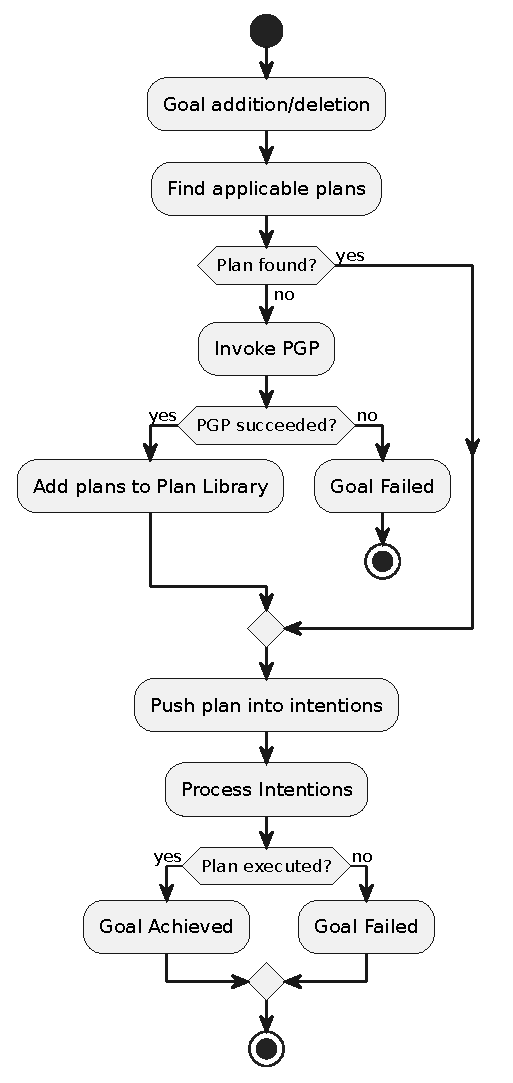
\includegraphics[
        width=0.42\linewidth,
    ]{figures/reactive-pgp.pdf}
    \caption{Simplified BDI control cycle that uses a reactive PGP to dynamically generate new plans at runtime.}
    \label{fig:reactive-pgp}
\end{figure}

\subsection{The PGP contract}\label{sec:pgp-contract}

The contract is built around five fundamental interfaces. 

The \texttt{GenerationConfig} interface encapsulates all configuration parameters needed for plan generation, allowing different generation approaches to specify their requirements without coupling to specific implementations.

The \texttt{GenerationResult} interface standardizes how generation outcomes are communicated back to the \ac{BDI} engine, whether successful or failed.

The \texttt{Generator} interface defines the core generation capability, abstracting away the specific mechanisms used to produce plans.

The \texttt{GenerationState} interface maintains the context throughout the generation process, tracking the plan generation goal, the associated \ac{PGP} identifier, and logging capabilities. 

The \texttt{GenerationStrategy} interface binds together a specific generator with its configuration. This design allows the \ac{BDI} engine to work with different generation approaches transparently, regardless of the kind of planners used and of how they are configured.

\begin{figure}
    \centering
    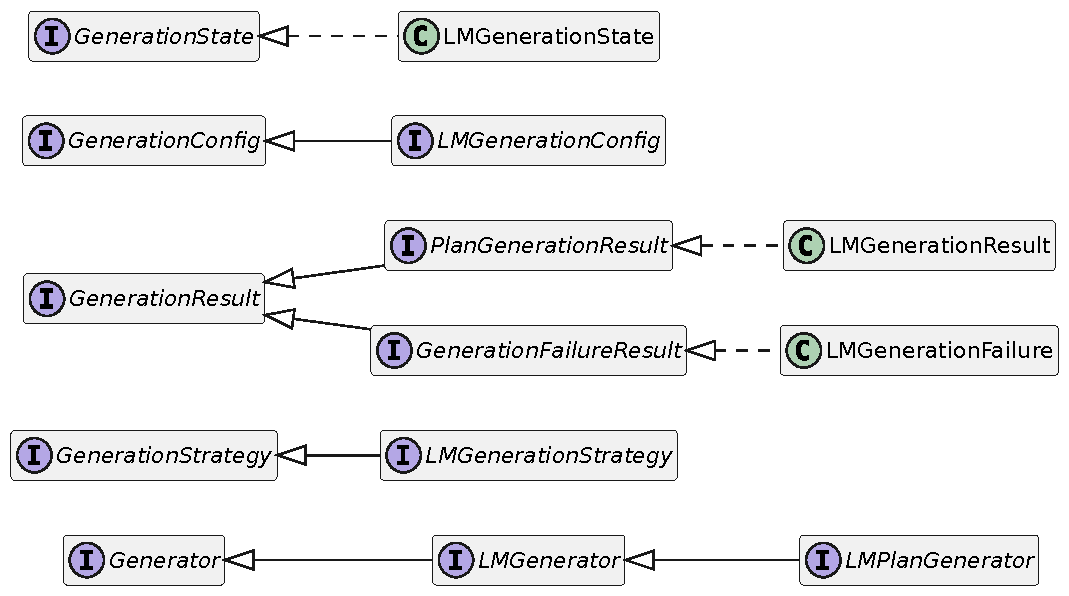
\includegraphics[width=0.8\textwidth]{figures/gen-interfaces.pdf}
    \caption{The interfaces that define the contract for plan generation exposed by the \ac{BDI} engine and the interfaces and classes that implement this contract for a LM-based PGP.}
    \label{fig:gen-interfaces}
\end{figure}

The LM-prefixed interfaces and classes, shown in~\cref{fig:gen-interfaces}, implement the language model-based \ac{PGP}.

The \texttt{LMGenerationConfig} extends the base configuration with LM-specific parameters including model identifiers, temperature settings, maximum token limits, and server endpoints for API communication.
%
In table~\ref{pgp-params} an outline of the configuration that the user can provide is given.

\begin{table}[htbp]
\centering
\begin{tabular}{|l|l|p{7cm}|}
\hline
\textbf{Parameter} & \textbf{Type} & \textbf{Description} \\
\hline
\texttt{model} & \texttt{String} & Specifies the language model to be used for plan generation (e.g., GPT-4, Claude, etc.) \\
\hline
\texttt{temperature} & \texttt{Double} & Controls the randomness of the generated output. Lower values produce more deterministic results, higher values increase creativity \\
\hline
\texttt{maxTokens} & \texttt{Int} & Maximum number of tokens that can be generated in the response, limiting the length of generated plans \\
\hline
\texttt{url} & \texttt{String} & The endpoint URL for the language model API service \\
\hline
\texttt{token} & \texttt{String} & Authentication token required to access the language model API \\
\hline
\texttt{requestTimeout} & \texttt{Duration} & Maximum time to wait for a complete API request-response cycle \\
\hline
\texttt{connectTimeout} & \texttt{Duration} & Maximum time to wait when establishing a connection to the API service \\
\hline
\texttt{socketTimeout} & \texttt{Duration} & Maximum time to wait for data transfer over an established connection \\
\hline
\texttt{contextFilter} & \texttt{ContextFilter} & Filter component that determines which contextual information should be included in the generation prompt \\
\hline
\texttt{promptBuilder} & \texttt{PromptBuilder} & Component responsible for constructing the prompt sent to the language model, including context formatting and instruction generation \\
\bottomrule
\end{tabular}
\caption{Configurable Parameters for the \ac{PGP}.}
\label{pgp-params}
\end{table}

The LM-based implementation provides two concrete types of generation results: \texttt{LMGenerationResult} for successful generations and \texttt{LMGenerationFailure} for error cases.
%
The success case handles both the generated plans and the admissible goals and beliefs invented by the \ac{LLM}, along with natural language descriptions.

The \texttt{LMGenerationState} extends the base state interface with chat history management.
%
This supports iterative refinement scenarios where the initial generation may be incomplete or require clarification.

The \texttt{LMPlanGenerator} implements the core generation logic through two key components: a \texttt{RequestHandler} responsible for sending requests to the language model according to the chosen provider, and a \texttt{Parser} that interprets the model's responses and extracts structured plan representations. 
%
This separation allows for independent evolution of the communication protocol and of the parsing logic.

The \texttt{LMGenerationStrategy} binds together the LM-specific generator and configuration.

\subsection{The Generation Manager}\label{sec:generation-manager}

The \texttt{GenerationManager} is the central component responsible for orchestrating the \ac{PGP} within the agent's control cycle.
%
Its role spans across initiating plan generation, tracking execution outcomes, managing failures, and maintaining the integrity of the dynamically generated plan library, delegating responsibilities to specialized strategy implementations. 
%
\Cref{fig:gen-manager} provides an overview of the core components and their interactions, which will be further discussed in the following sections.

\begin{figure}
    \centering
    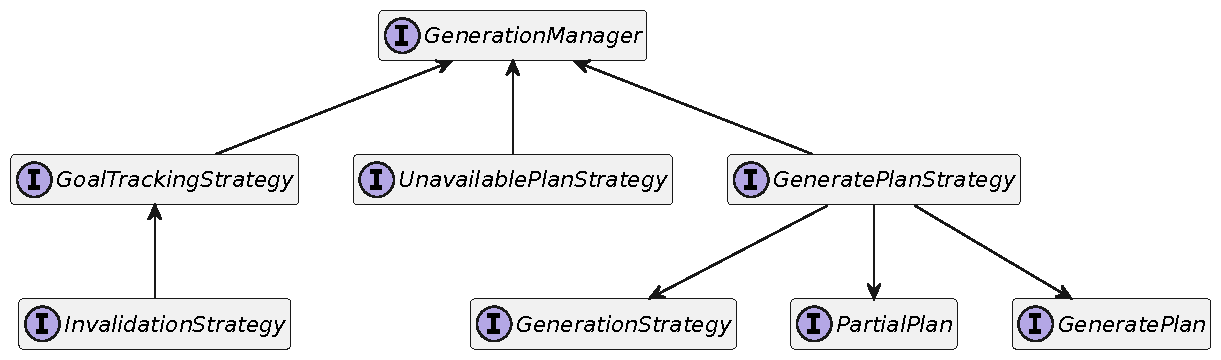
\includegraphics[width=\textwidth]{figures/gen-manager.pdf}
    \caption{Components of the \texttt{GenerationManager}, which orchestrates the \ac{PGP}.}
    \label{fig:gen-manager}
\end{figure}

\subsubsection{Generation Goals}

The \texttt{GeneratePlan} goal serves as the primary interface between the \ac{BDI} control cycle and the plan generation process.
%
This goal encapsulates a request for plan generation, storing both the target goal for which plans should be generated and optional configuration parameters that control the generation process.
%
When a \texttt{GeneratePlan} goal is encountered during the execution of an intention, it is processed by the \texttt{GenerationManager}.
%
The system first checks if a generation strategy is available - if not, it returns a failure feedback indicating that plan generation cannot proceed without a configured strategy.
%
This design ensures that agents can operate with or without plan generation capabilities, providing backward compatibility with traditional BDI systems.

The execution of a \texttt{GeneratePlan} goal involves several steps:
%
\begin{inlinelist}
    \item the generation strategy is optionally updated with the provided configuration,
    \item a generation state is initialized with the current agent context, and finally
    \item the actual plan generation request is made to the generation strategy.
\end{inlinelist} 
%
This process integrates with the existing \ac{BDI} control cycle, allowing generated plans to be available in the plan library when the generation completes.

\subsubsection{Partial Plans}

Plans generated by the \ac{PGP} are stored as partial plans, which maintain references to their generation context and can be dynamically invalidated by using a plan invalidation mechanism.
%
Unlike traditional plans in \ac{BDI} systems, partial plans hold information about their origin, specifically the generation goal that created them and the configuration used during generation.
%
When a partial plan is scheduled in an intention, only the goals being tracked are included if there are any, otherwise all the goals are used to create an activation record as in standard \ac{BDI} plans.
%
When determining if a partial plan is applicable to a given event, the system checks the standard trigger matching and guard conditions ignoring the source of the beliefs \footnotemark{}.
%
\footnotetext{
    Agents that employ a generation strategy currently ignore belief sources when unifying with the belief base.
    %
    This limitation exists because sources cannot be reliably added to generated beliefs automatically, and the LLM is not prompted to annotate beliefs with sources to avoid increasing prompt complexity.
}

\subsubsection{Tracking the Generated Goals}\label{sec:tracking-goals}

The system implements a goal tracking mechanism to monitor the execution of goals within generated partial plans.
%
This is achieved through the \texttt{TrackGoalExecution} goal type, which wraps the actual goals that need to be executed and provides hooks for verifying their success or failure.
%
The tracking mechanism serves multiple purposes: it enables the system to detect when generated plans fail to achieve their intended outcomes, and it provides feedback that is used for debugging and that can potentially be used to improve future plan generation.

The \texttt{GoalTrackingStrategy} manages the tracked goals, replacing them with their actual counterparts during execution and checking their results. 
%
When a tracked goal executes successfully, the system updates the plan library to ``untrack'' the goal.
%
When all tracking goals of a partial plan get removed, then the generated plan can be considered as successfully executable.
%
This of course does not mean that the plan achieves the goal for which it was generated, since no verification mechanism is in place, nor that it does so optimally. 
%
The tracking mechanism also handles failure cases by triggering the invalidation strategy when tracked goals fail. 
%
This ensures that plans that prove ineffective in practice are removed from the plan library, preventing the agent from repeatedly attempting unsuccessful approaches. 
%
In principle this can also be used to trigger a plan repair mechanism since it also provides the execution feedback of the failed goal being tracked.

\subsubsection{Handling Plan Unavailability}\label{sec:plan-unavailability}

The PGP trigger strategy determines when plan generation should be initiated during the control cycle. 
%
The system supports both the on demand and reactive approaches described in~\cref{sec:triggering-generative-process}, where plan generation is triggered by the \texttt{generate\_plan} action or when the agent encounters situations for which no applicable plans exist.
%
The \texttt{UnavailablePlanStrategy} interface intercepts plan selection failures and evaluates whether they can be resolved through dynamic plan generation.
%
The system distinguishes between the absence of relevant plans and the presence of relevant but inapplicable plans. 
%
The \texttt{UnavailablePlanStrategyImpl} implements this logic by first categorizing the type of unavailability and then applying appropriate resolution strategies.
%
When no plans are found for a given event trigger, the system checks if the event represents an achievement goal.
%
If so, it creates a new $p_{genex}$ plan (\S~\ref{sec:reactive-pgp}) using the \texttt{GenerationPlanBuilder}, adding it to the plan library along with the \inlineAsl{missing\_plan\_for(G)} belief and an event to trigger the generation process.
%
For cases where relevant plans exist, but none are applicable due to failed preconditions, the system provides detailed feedback about the applicability failures.
%
This includes logging information about which guards failed and why, enabling developers and potentially the agent itself to understand the reasons for plan rejection.

\subsubsection{The Plan Invalidation Mechanism}\label{sec:plan-invalidation}

The plan invalidation mechanism has the responsibility of maintaining the integrity of the generated plan library by removing plans that have proven ineffective. 
%
The current \texttt{InvalidationStrategy} implements this mechanism by selectively removing partial plans from the plan library when they are associated with failed goal executions.
%
The system specifically targets partial plans for removal, preserving manually authored plans and cleaning up dynamically generated content that has proven problematic.

There are no mechanisms in place to prevent unchecked growth of the plan library.
%
To prevent this issue, an \texttt{InvalidationStrategy} could also include mechanisms to ``forget'' plans if they are not used over time, to rank them and periodically remove the least important ones, to factorize them or to offload them to an external storage once a threshold is reached.

\subsubsection{Plan Generation Strategy}\label{sec:plan-gen-strategy}

\Cref{fig:plan-gen} shows an overview of the \texttt{GeneratePlanStrategy} interface.
%
It handles the initial setup and delegates the actual generation request to a chosen strategy.
%
It then uses the \texttt{GenerationResultBuilder} interface to construct \\ \texttt{PlanGenerationResult}s from successful plan generations, that can be integrated transparently into the \ac{BDI} engine.
%
Each of the three \texttt{Updater}s within the result builder handles a specific aspect of integrating the generated content into the agent's context.

\begin{figure}
    \centering
    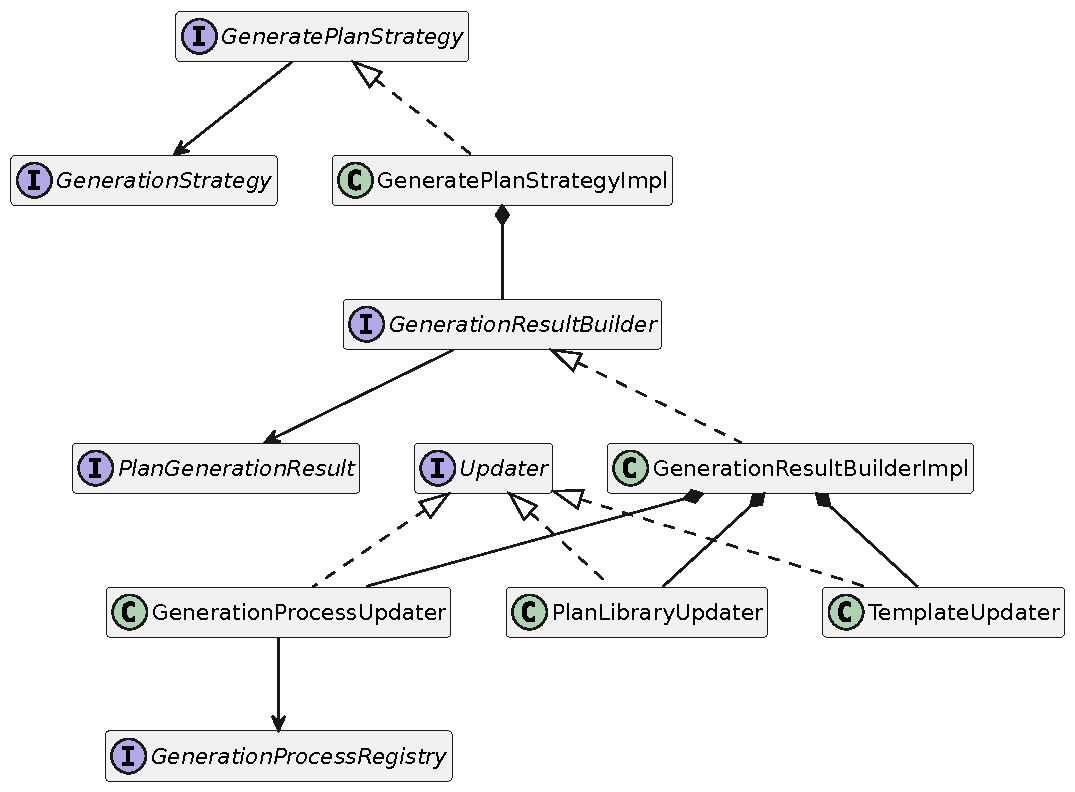
\includegraphics[width=0.75\textwidth]{figures/plan-gen.pdf}
    \caption{Components of the \texttt{GeneratePlanStrategy}, which invokes the generation strategy provided by the user and updates the result to the agent that requested the generation.}
    \label{fig:plan-gen}
\end{figure}

The \texttt{TemplateUpdater} class manages the integration of newly generated admissible beliefs and goals into the agent's context.
%
For admissible beliefs, it merges the existing beliefs with newly generated ones, using the rule head functor as a unique identifier to prevent duplicates.
%
Analogously, for admissible goals, it combines existing and new goals using the trigger value functor to distinguish them.

The \texttt{PlanLibraryUpdater} handles the integration of newly generated plans into the agent's plan library. 
%
It processes each generated plan by wrapping the plan goals with a \texttt{TrackGoalExecution}.
%
The updated plans are then merged with the existing plan library.
%
Newer plans overwrite existing ones with the same trigger and context.

The \texttt{GenerationProcessUpdater} manages a registry of generation processes, updating their state according to generation results.
%
This underlying \\ \texttt{GenerationProcessRegistry} is implemented as a map, linking each goal generation request to its corresponding generation state.
%
The use of a registry potentially allows to handle long-running \acp{PGP}, including those involving \acp{LLM} that may require multiple interaction turns.

\section{Logging System}\label{sec:logging-system}

As part of the development of the \ac{PGP}, a logging system was introduced in \jakta{} to ease debugging and to extract structured data from execution traces as part of the experimental evaluation.
%
The logging system is based on the interfaces \texttt{LogEventContext} and \texttt{LogEvent}.
%
The first interface acts as a wrapper of \texttt{LogEvent}s and provides information used to unequivocally identify each event with the identifier of the \ac{MAS} execution, the identifier of the agent and the identifier of the running \ac{PGP}, if they are relevant for the event.
%
\texttt{LogEvent} is the base interface from which all other log events extend. In \cref{fig:jakta-log-event} the base hierarchy is shown. There are three main kinds of events:

\begin{itemize}
    \item \texttt{AgentEvent} references log events generated by each agent, relative to its internal mechanics and its data structures. 
    %
    For example, this includes events related to the selection, addition or removal of intentions, plans or events. In~\cref{fig:jakta-log-event} and~\cref{fig:agent-event} all the logged events are shown.
    \item \texttt{EnvironmentEvent} references the effects that are applied to the environment after the execution of the control cycle of an agent.
    %
    This includes for example receiving, sending or broadcasting messages. 
    %
    In~\cref{fig:environment-change} all the log events relative to the environment provided by the BDI engine are shown. 
    %
    By extending the interface, new kind of environmental conditions can be logged from user-provided environments.
    \item \texttt{ExecutionFeedback} references events relative to the result of the execution of the sense-reason-act cycle. 
    %
    This includes whether relevant or applicable plans are not found during the deliberation or if the execution of an action fails in the action phase. 
    %
    In~\cref{fig:execution-feedback-goals} and~\cref{fig:execution-feedback-pgp} all the feedback events provided by the BDI engine are shown. 
    %
    By extending the interface, the user can record new kinds of feedback as a result of the execution of custom actions.
\end{itemize}

\begin{figure}
    \centering
    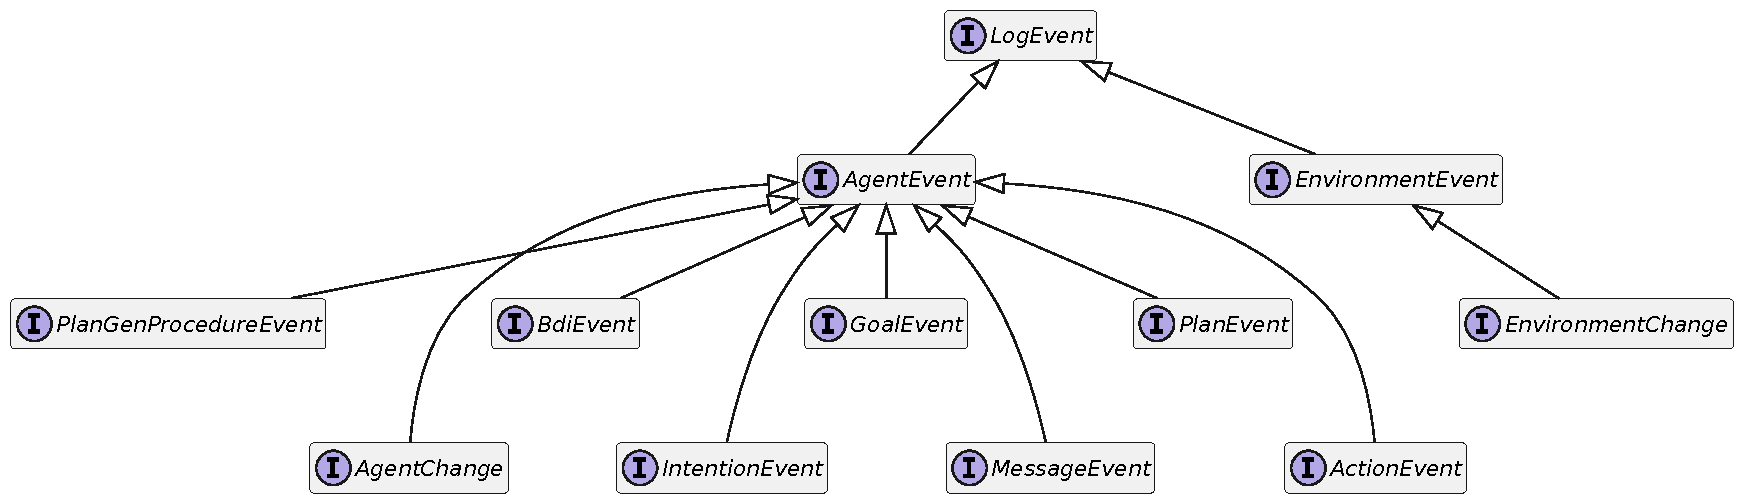
\includegraphics[width=\textwidth]{figures/log-event.pdf}
    \caption{\texttt{LogEvent} interface hierarchy.}
    \label{fig:jakta-log-event}
\end{figure}

\begin{figure}
    \centering
    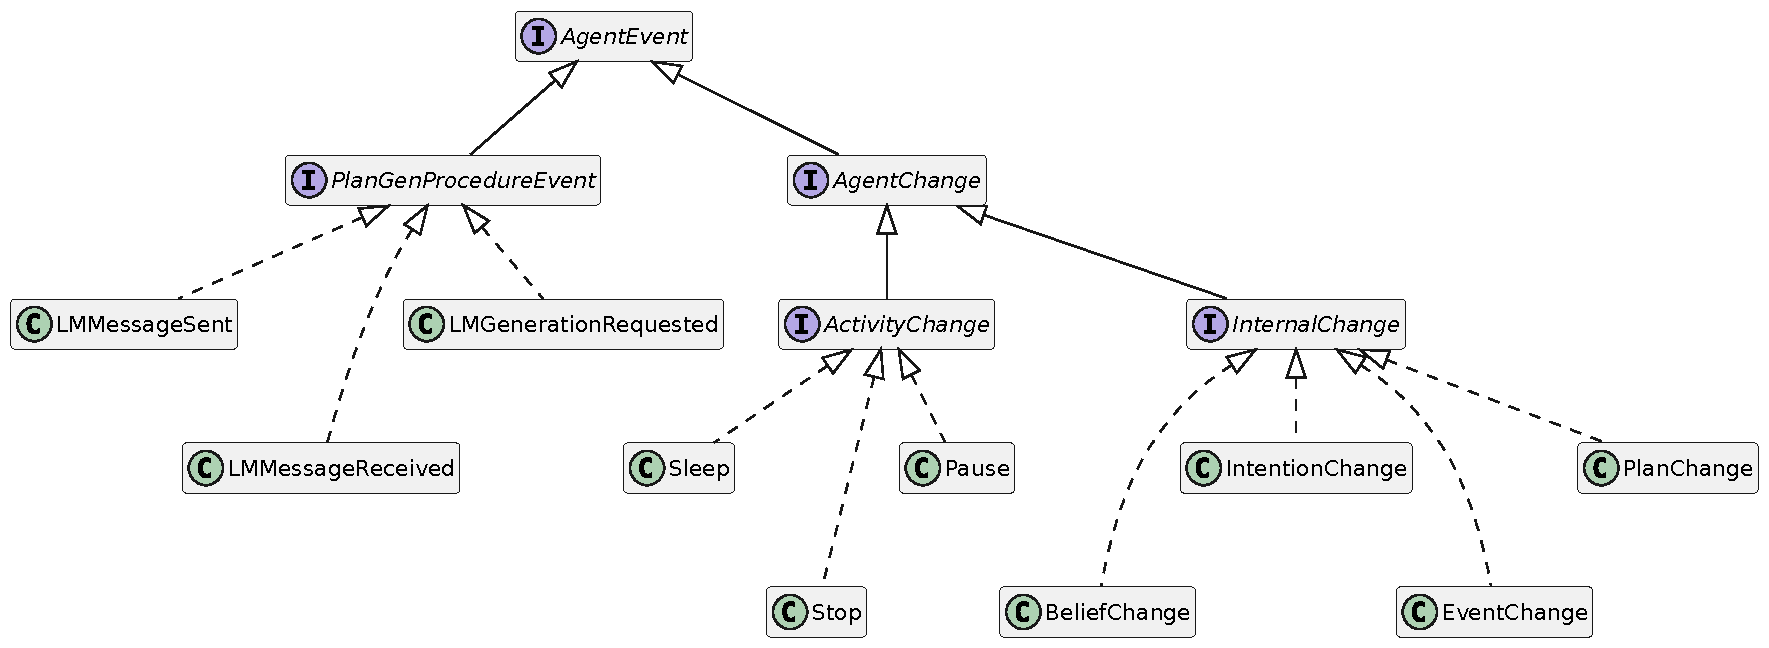
\includegraphics[width=\textwidth]{figures/agent-event.pdf}
    \caption{\texttt{AgentEvent} interface hierarchy.}
    \label{fig:agent-event}
\end{figure}

\begin{figure}
    \centering
    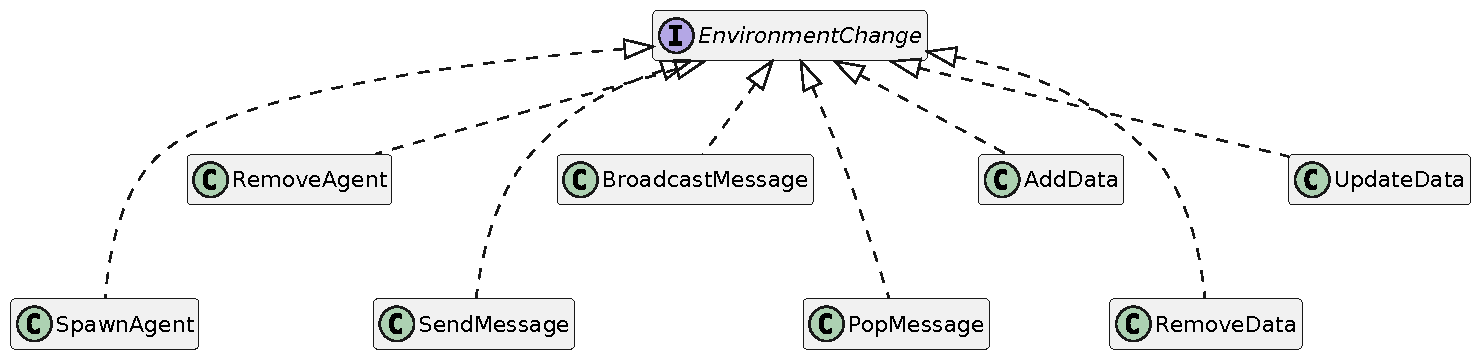
\includegraphics[width=\textwidth]{figures/environment-change.pdf}
    \caption{\texttt{EnvironmentChange} interface hierarchy.}
    \label{fig:environment-change}
\end{figure}

\begin{figure}
    \centering
    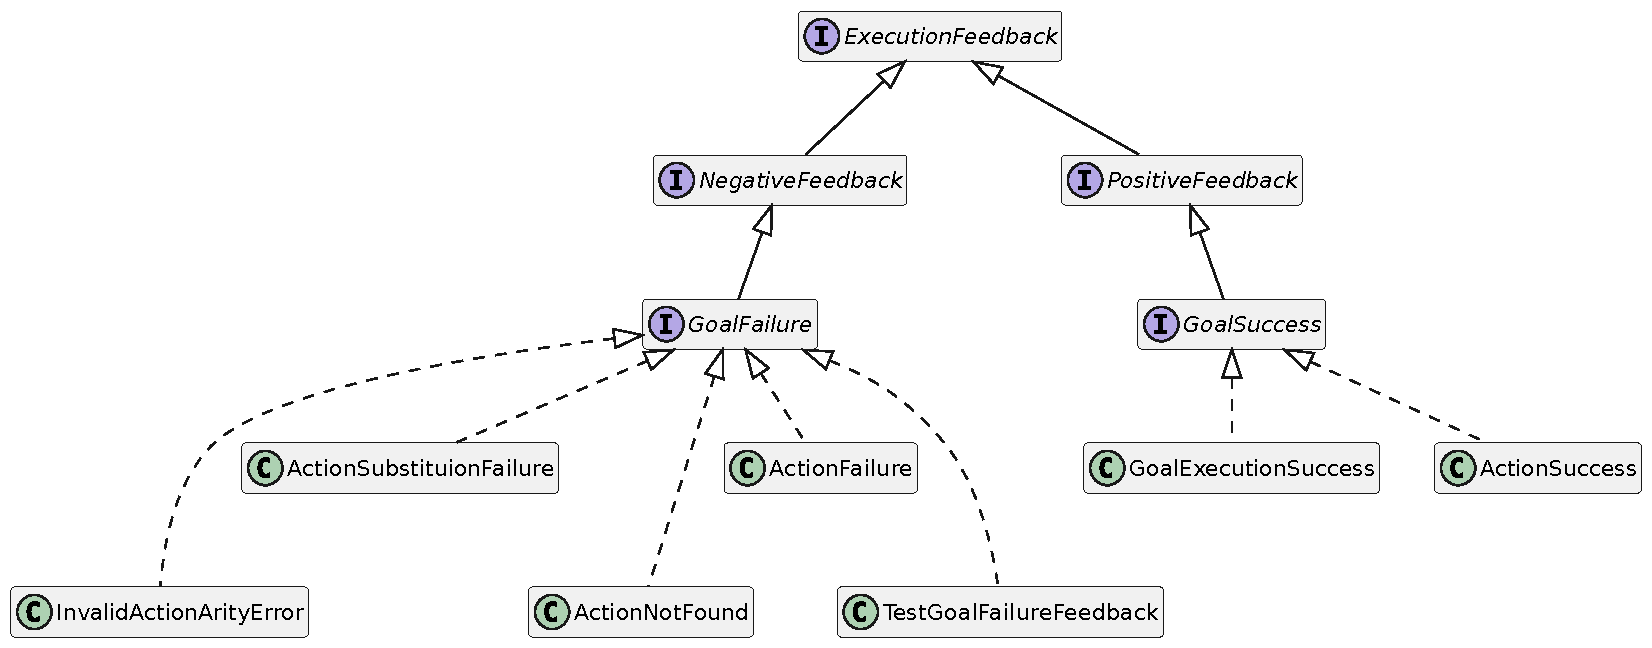
\includegraphics[width=\textwidth]{figures/execution-feedback.pdf}
    \caption{\texttt{ExecutionFeedback} interface hierarchy considering only goals' results.}
    \label{fig:execution-feedback-goals}
\end{figure}

\begin{figure}
    \centering
    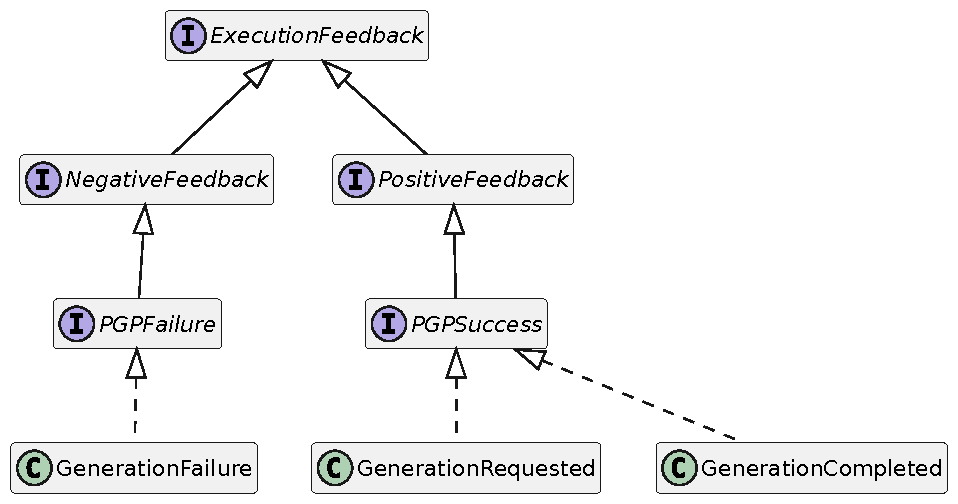
\includegraphics[width=0.7\textwidth]{figures/exec-feed-pgp.pdf}
    \caption{\texttt{ExecutionFeedback} interface hierarchy considering only PGPs' results.}
    \label{fig:execution-feedback-pgp}
\end{figure}

The \texttt{JaktaLogger} interface provides the starting point from which the loggers are defined, and provides a set of functions to log strings or objects, according to the chosen log level. 
%
It is implemented by the \texttt{MasLogger}, \texttt{AgentLogger} and \texttt{PgpLogger} interfaces.

When logging is enabled, a \texttt{MasLogger} instance is created during the initialization of the \ac{MAS}.
%
Subsequently, each agent is assigned its own \texttt{AgentLogger}.
%
A \texttt{PgpLogger} is instantiated by the generation manager when a new generation state is initialized, specifically during the processing of a \texttt{GeneratePlan} goal.

The \texttt{MasLogger} is responsible for logging \texttt{EnvironmentEvent}s, which include environmental effects and user-defined environment events.
%
The \texttt{AgentLogger} logs all \texttt{AgentEvent}s except those of type \texttt{PlanGenProcedureEvent}, which are handled exclusively by the \texttt{PgpLogger}.

Both \texttt{MasLogger} and \texttt{AgentLogger} are also responsible for logging events of type \texttt{ExecutionFeedback}.

Logging behavior is governed by the \texttt{LoggingConfig} class, which stores configuration flags such as whether to log to the console, to one or more files, or to a remote server. 
%
If a \ac{MAS} is created without this configuration, then the application will not log anything.

\section{Generative Process Pipeline}\label{sec:generative-pipeline}

This section presents the five core components that are used to implement \ac{LLM}-based generation strategies.
%
\textit{Context filters} (\S~\ref{sec:context-filters}) retain relevant knowledge, \textit{formatters} (\S~\ref{sec:formatters}) encode this knowledge into \ac{LLM} prompts, and \textit{parsers} (\S~\ref{sec:parsers}) decode structured responses. 
%
\textit{Request handlers} (\S~\ref{sec:request-handlers}) manage \ac{LLM} interactions, while \textit{plan generators} (\S~\ref{sec:plan-generators}) orchestrate the overall workflow.

\subsection{Context filters}\label{sec:context-filters}

A context filter implements the interface \texttt{ContextFilter}, which takes in input an \texttt{ExtendedAgentContext} and returns a filtered \texttt{ExtendedAgentContext}. 
%
The extended agent context includes both the agent context and all the additional data that might be used to build the prompt of a \ac{LLM}, such as the external actions provided by the environment or the initial goal provided by the user.
%
In~\cref{sec:custom-filters} an example filter definition is shown.
%
Context filters control what information reaches the language model, reducing information overload and improving response quality.

\subsection{Formatters}\label{sec:formatters}

A formatter implements the \texttt{Formatter} interface and transforms internal data structures into human-readable string representations for LLM consumption, logging and debugging. 
%
The system includes built-in formatters for encoding agent and environment context in LLM prompts.
%
As an example,~\cref{lst:action-formatter} shows how the action formatter transforms action objects into descriptive strings that include the action signature, parameter names, and optional purpose description.

\begin{lstlisting}[
    basicstyle=\scriptsize\ttfamily,
    breaklines=true,
    language=Kotlin,
    label={lst:action-formatter},
    captionpos=b,
    caption={Implementation of the action formatter that converts \texttt{Action}s into human-readable string representations for LLM prompts.}
]
val actionsFormatter = Formatter<Action<*, *, *>> { action ->
    buildString {
        val signature = action.actionSignature
        append(signature.name, "(")
        append(
            signature.parameterNames.takeIf { it.isNotEmpty() }
                ?.joinToString { it.capitalize() }
                ?: (1..signature.arity).joinToString { "Parameter$it" }
        )
        append(")")
        action.purpose?.let { append(": $it") }
    }.dropWordsWithTrailingNumbers()
}
\end{lstlisting}

\subsection{Parsers}\label{sec:parsers}

A parser implements the \texttt{Parser} interface and converts the text generated by the \ac{LLM} into structured internal representations. 
%
The parser implemented for the prototype extracts YAML code blocks from input text.
%
It attempts to decode content as either \texttt{PlanData} or lists of \texttt{TemplateData}. 
%
Its responsibilities include processing different template types (beliefs and goals), validating the parsed structures, and accumulating any parsing errors.
%
\Cref{fig:parser-result} shows both the type of errors that can be accumulated by the parser and the kind of results it can return.
%
The final result aggregates successfully parsed plans, admissible beliefs, and admissible goals in the \texttt{NewResult} class, along with parsing errors, if there any, or returns an \texttt{EmptyResponse} if no valid content was extracted.

\begin{figure}
    \centering
    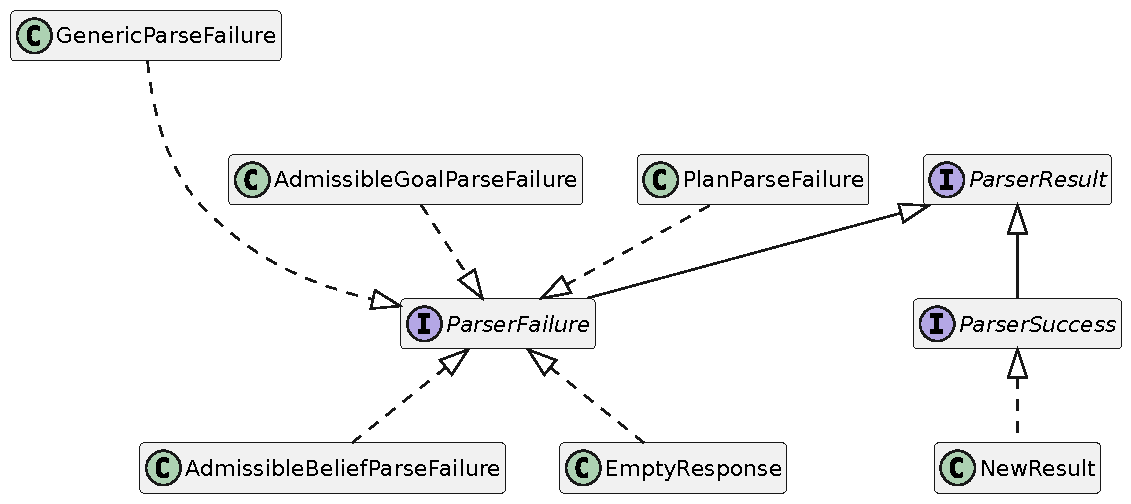
\includegraphics[width=\textwidth]{figures/parser-result.pdf}
    \caption{Set of interfaces that handle the parser's results.}
    \label{fig:parser-result}
\end{figure}

\subsection{Request Handlers}\label{sec:request-handlers}

The \texttt{RequestHandler} interface encapsulates the configuration, communication, and delegation needed to carry out text-based completions with \acp{LLM}, returning structured results that the rest of the pipeline can consume.

A text generation request is built from the current generation configuration and state.
%
Once the request is ready, it is sent to a \texttt{RequestProcessor}.
%
The \texttt{RequestProcessor} handles low-level communication with the model through an OpenAI-compliant API and passes the raw response through a \texttt{Parser} and translates the \texttt{ParserResult} into a structured \texttt{RequestResult}.

The \texttt{RequestResult} interface represents whether a request had success or not.
%
If the request is successful a \texttt{NewRequestResult} object is created, which encapsulates parsed plans (\texttt{NewPlan}), admissible goals, beliefs, and any potential parsing errors in the \texttt{NewResult} object. 
%
A \texttt{NetworkRequestFailure} is returned instead if there are problems such as timeouts or invalid responses.

\subsection{Plan Generators}\label{sec:plan-generators}

As it is shown in \cref{fig:gen-strat} the \texttt{LMGenerator} interface defines the high-level abstraction that is used by the \texttt{LMGenerationStrategy} to handle generation requests. 
%
It relies on the \texttt{RequestHandler} to issue requests and parse results, while also logging relevant messages and updating the generation state.

\begin{figure}
    \centering
    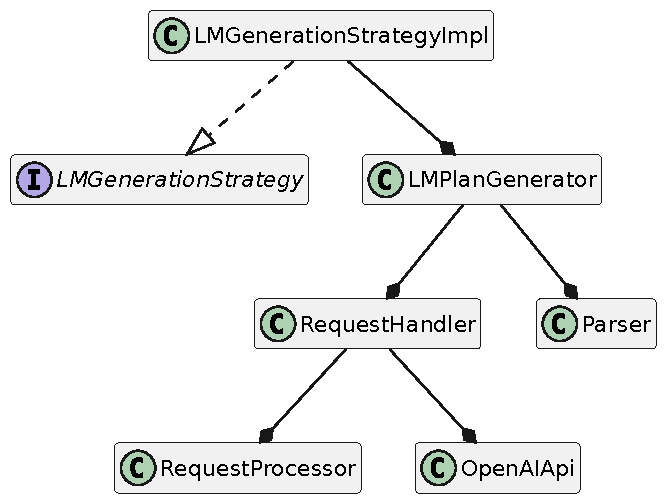
\includegraphics[width=0.5\textwidth]{figures/gen-strat.pdf}
    \caption{Set of classes that compose a LLM-based plan generation strategy.}
    \label{fig:gen-strat}
\end{figure}

\section{Generative Agent Specification}\label{sec:generative-agent-spec}

This section describes how to declare and configure generation strategies for use by the PGP, building upon the components introduced in the previous section.
%
The configuration process is structured in several areas.
%
Prompt templates can be defined using a Kotlin \ac{DSL} (\S~\ref{sec:prompt-templates}), while the scope and parameters that define the generation strategy are selected through dedicated configuration mechanisms (\S~\ref{sec:gen-strat}).
%
For enhanced performance, custom filters serve to regulate information flow to the LLM (\S~\ref{sec:prompt-templates}), and natural language documentation provides helpful operational hints (\S~\ref{sec:write-doc}).
%
The specification of on-demand generation goals offers additional flexibility (\S~\ref{sec:on-demand-goals}), and custom log events allow to debug the generation process and support automatic evaluation procedures (\S~\ref{sec:custom-log-events}).

\subsection{Implementing Custom Filters}\label{sec:custom-filters}

As the size of the belief base of an agent, its set of actions and available plans grows, it becomes impractical and performance-degrading to keep all that information in the context. 
%
For that reason, mechanisms to filter out information are needed.
%
Custom filters provide a mechanism to control what information from the \ac{BDI} agent state is presented to the \ac{LLM} during plan generation. 

The filtering mechanism operates on an \texttt{ExtendedAgentContext} structure that encapsulates the complete agent state, including the initial goal, the current context with beliefs and plans, and available external actions.

Effective filtering significantly improves the performance of \ac{LLM}-based \ac{BDI} agents by:
%
\begin{inlinelist}
    \item reducing the token count in prompts, leading to faster response times and lower computational costs,
    \item decreasing the cognitive load on the \ac{LLM} by presenting only relevant information, and
    \item minimizing the risk of the \ac{LLM} being distracted by irrelevant or contradictory information.
\end{inlinelist}

When implementing custom filters, the trade-off between information completeness and performance must be carefully balanced. 
%
Overly aggressive filtering may remove crucial information that could lead to better plans, while insufficient filtering may degrade performance without providing meaningful benefits.

\lstinputlisting[
    label={lst:default-filter},
    caption={Default context filter implementation that removes meta-plans and failure-handling plans to streamline the LLM context for plan generation.},
    language=Kotlin,
    basicstyle=\scriptsize\ttfamily,
    captionpos=b,
    mathescape=false
]{listings/default-filter.kt}

The built-in filter, shown in~\cref{lst:default-filter}, removes the special generation plans that are automatically created when no applicable plan exists for a goal, as described in~\cref{sec:reactive-pgp}. 
%
These meta-plans are internal mechanisms that would confuse the \ac{LLM} during plan generation and are thus omitted.

\subsection{Defining Prompt Builders}\label{sec:prompt-templates}

The \ac{PGP} requires incorporating dynamic content, structured data, and contextual information. 
%
Traditional string concatenation approaches become unwieldy and error-prone when dealing with prompts containing nested hierarchies and conditional content. 
%
A Kotlin \ac{DSL} was developed to address this challenge and enable declarative prompt construction while maintaining type safety and readability.
%
In~\cref{lst:prompt-with-hints} an example of use of the \ac{DSL} is shown.

The \texttt{PromptScope} class serves as the primary builder for prompt construction.
%
It maintains an internal list of \texttt{PromptSection} objects and provides methods for adding different types of content.
%
This design separates content from presentation, allowing the same section to be rendered at different heading levels depending on its position in the hierarchy.

The \ac{DSL} provides several directives for adding content to user or system prompts:
%
\begin{inlinelist}
    \item \texttt{section}: creates a titled section with nested content,
    \item \texttt{fromFile}: includes content from resource files,
    \item \texttt{fromFormatter}: applies formatting functions to data, and
    \item \texttt{fromString}: adds literal text content.
\end{inlinelist}
%
Providing both user and system \acp{DSL} reflects how \acp{LLM} differentiate between system instructions and user queries and allows building better prompts.
%
This separation of concerns improves code clarity, prevents accidental misuse of the two roles, and aligns with best practices in prompt engineering.

\lstinputlisting[
    label={lst:prompt-with-hints},
    caption={Example of a user prompt template, which is populated at runtime according to the state of the agent and the content of static files.},
    language=Kotlin,
    basicstyle=\scriptsize\ttfamily,
    captionpos=b,
    mathescape=false
]{listings/prompt-spec.kt}

\subsection{Declaring the Generation Strategy}\label{sec:gen-strat}

One of the most relevant aspects of the specification involves selecting an appropriate generation strategy and defining its scope and configuration parameters. 
%
The framework implements a \ac{LLM}-based generation strategy which leverages the pipeline components detailed in~\cref{sec:generative-pipeline}.
%
After selecting a generation strategy and configuring its parameters, the scope where the strategy applies can be defined. The system supports three hierarchical declaration levels, each offering different application scopes:
%
\begin{inlinelist}
    \item \ac{MAS}-Level: defines the default generation strategy for the entire Multi-Agent System (\cref{lst:mas-level-gen-strat}),
    \item agent-level: specifies generation strategies for individual agents, overriding MAS-level settings (\cref{lst:agent-level-gen-strat}), and
    \item plan-level: sets generation strategies for specific plans, taking precedence over both agent and MAS-level configurations (\cref{lst:plan-level-gen-strat}).
\end{inlinelist}
%
This hierarchical structure operates on a specificity-based override system. 
%
The precedence flows from plan-level (the highest priority) to agent-level (medium priority) to MAS-level (the lowest priority), to make sure that the most specific configuration always governs the behavior.
%
When conflicts arise between different declaration levels, the system employs a granular resolution mechanism.
%
Rather than replacing entire configuration blocks, individual parameters are overwritten based on the hierarchy.
%
This allows for fine-grained control where, for example, an agent might inherit most parameters from the MAS level while only modifying specific settings such as temperature or max tokens.

\lstinputlisting[
    label={lst:mas-level-gen-strat},
    caption={Example of a generation strategy declared at the MAS level.},
    language=Kotlin,
    basicstyle=\scriptsize\ttfamily,
    captionpos=b,
    mathescape=false
]{listings/mas-level-gen-strat.kt}

\lstinputlisting[
    label={lst:agent-level-gen-strat},
    caption={Example of a generation strategy declared at the agent level.},
    language=Kotlin,
    basicstyle=\scriptsize\ttfamily,
    captionpos=b,
    mathescape=false
]{listings/agent-level-gen-strat.kt}

\lstinputlisting[
    label={lst:plan-level-gen-strat},
    caption={Example of a generation strategy declared at the plan level.},
    language=Kotlin,
    basicstyle=\scriptsize\ttfamily,
    captionpos=b,
    mathescape=false
]{listings/plan-level-gen-strat.kt}

\subsection{Writing the Documentation}\label{sec:write-doc}

The \ac{DSL} provided by \jakta{} has been extended with additional syntactical constructs, in order to allow programmers to provide hints, as explained in~\cref{sec:writing-generative-agent-specs}.
%
The new entries of the \ac{DSL} are:
\begin{inlinelist}
    \item the \texttt{.meaning\{\ldots\}} blocks, which can be used to tag \emph{actual} goals, beliefs, or actions with their intended meaning, via a postfix syntax; and
    \item the \texttt{admissible\{\ldots\}} blocks, which can be used to tag \emph{admissible} goals or beliefs with their intended meaning, via a prefix syntax.
\end{inlinelist}
%
In both cases, the meaning is expressed as a string, attained via string interpolation, which in turn may include the functor and the arguments.
%
The strings are then exploited by the \ac{PGP} to generate the prompt for the \ac{LLM} through formatters.

An example of use of the new constructs is shown in~\cref{lst:hints-spec}.

\lstinputlisting[
    label={lst:hints-spec},
    caption={Example of a \jakta{} agent extended with natural-language descriptions},
    language=Kotlin,
    basicstyle=\scriptsize\ttfamily,
    captionpos=b,
    mathescape=false
]{listings/hints-spec.kt}

Moreover, the \texttt{remark} method can be used to provide the LLM with additional constraints or suggestions to further guide the generative process.
%
The additional instructions are added to the prompt in a dedicated section.

\subsection{Specifying on-demand Generation Goals}\label{sec:on-demand-goals}

In~\cref{lst:on-demand-generation} an example of agent specification that explicitly uses the on-demand \ac{PGP} approach is shown. 
%
The agent has the goal of printing the numbers from zero to ten, but instead of providing a pre-written plan with specific implementation details, the plan body contains only a call to the \texttt{generate\_plan} action. 
%
This provides an example of how programmers can delegate the actual plan generation to the underlying \ac{LLM} while maintaining control over when and under what conditions the generation should occur.
%
When the agent needs to achieve the goal \texttt{print\_numbers(0, 10)}, it will execute the corresponding plan, which triggers the \ac{PGP} to generate an appropriate implementation plan. 
%
The configured \ac{LLM} will receive the natural language description ``Print the numbers from 0 to 10'' along with the specific context and generate a concrete plan that implements the required functionality. 

\lstinputlisting[
    label={lst:on-demand-generation},
    caption={Example of a \jakta{} agent that will try to generate a plan to print the numbers from zero to ten using the provided generation strategy.},
    language=Kotlin,
    basicstyle=\scriptsize\ttfamily,
    captionpos=b,
    mathescape=false
]{listings/on-demand-spec.kt}

\subsection{Defining Custom Log Events}\label{sec:custom-log-events}

While the logging system described in \cref{sec:logging-system} covers the standard BDI engine operations, applications might require domain-specific logging capabilities that capture the unique characteristics of their problem domain.
%
Custom environments that extend the \texttt{Environment} interface can benefit from implementing and logging domain-specific events that capture when the system reaches particular states of interest. 
%
These specialized events provide more granular insight into the environment's behavior than generic state transitions.
%
Analogously, when creating custom actions, the \texttt{addFeedback} method from the \texttt{Action} interface enables the provision of detailed, domain-specific \texttt{ExecutionFeedback} log events that can provide richer diagnostic information of action outcomes beyond simple binary success or failure indicators.

\lstinputlisting[
    label={lst:custom-feedback-spec},
    caption={Implementation of the \texttt{move} action, which provides a more specific feedback than the default \texttt{GenericActionSuccess} when the action completes successfully.},
    language=Kotlin,
    basicstyle=\scriptsize\ttfamily,
    captionpos=b,
    mathescape=false
]{listings/custom-feedback-spec.kt}

These user-provided log events serve multiple purposes: they streamline experimentation workflows, support monitoring and debugging capabilities, and can provide structured input to aid \acp{LLM} in plan repair and refinement.
%
As an example the \texttt{move} action, which is shown in~\cref{lst:custom-feedback-spec}, provides specific feedback based on movement outcomes, rather than returning generic success messages. 
%
When the action executes successfully, it returns a \texttt{MoveActionSuccess} object containing movement details. When an agent reaches its home location, the system generates an \texttt{ObjectReachedEvent} providing feedback about this outcome.
%
The feedback of the action is used during the evaluation of the explorer bot example in \cref{chap:evaluation} to assess whether a \ac{PGP} completes the requested goal, by examining the execution trace for the presence or absence of the \texttt{ObjectReachedEvent}.

\chapter{Evaluation}\label{chap:evaluation}

This chapter evaluates the reactive PGP implementation within the ``Explorer Robot'' domain, defined in~\cref{sec:exp-robot}.
%
The agent-based application used for the evaluation features specifications enhanced by natural language descriptions, first conceptualized in~\cref{sec:writing-generative-agent-specs} and then implemented in~\cref{sec:generative-agent-spec}.
%
The experimental methodology employed to assess the agent's behavior is presented in~\cref{sec:exp-methodology} and the resulting outcomes are discussed in~\cref{sec:exp-results}.

\section{The explorer robot application}\label{sec:exp-robot}

In the explorer robot domain, an agent acts as an explorer (\S~\ref{sec:explorer-agent}) and has the objective of reaching home within a bidimensional grid world environment (\S~\ref{sec:explorer-environment}), where it can perceive obstacles in its immediate surroundings and move in the eight cardinal directions.
%
\Cref{fig:environment-model} shows the environment model.

\begin{figure}
    \centering
    \begin{subfigure}[c]{0.48\linewidth}
        \centering
        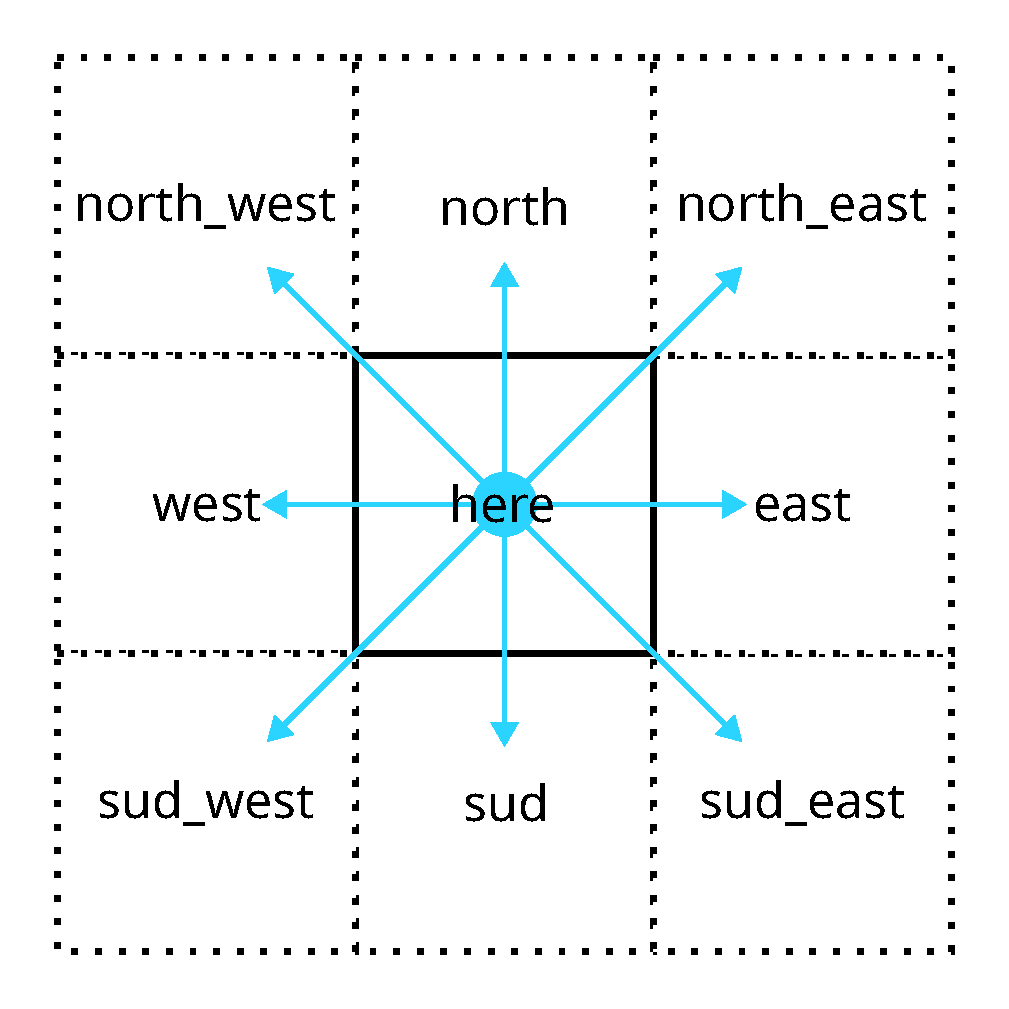
\includegraphics[height=4.5cm]{figures/directions.pdf}
        \caption{Nine admissible directions}
        \label{fig:directions}
    \end{subfigure}
    \hfill
    \begin{subfigure}[c]{0.48\linewidth}
        \centering
        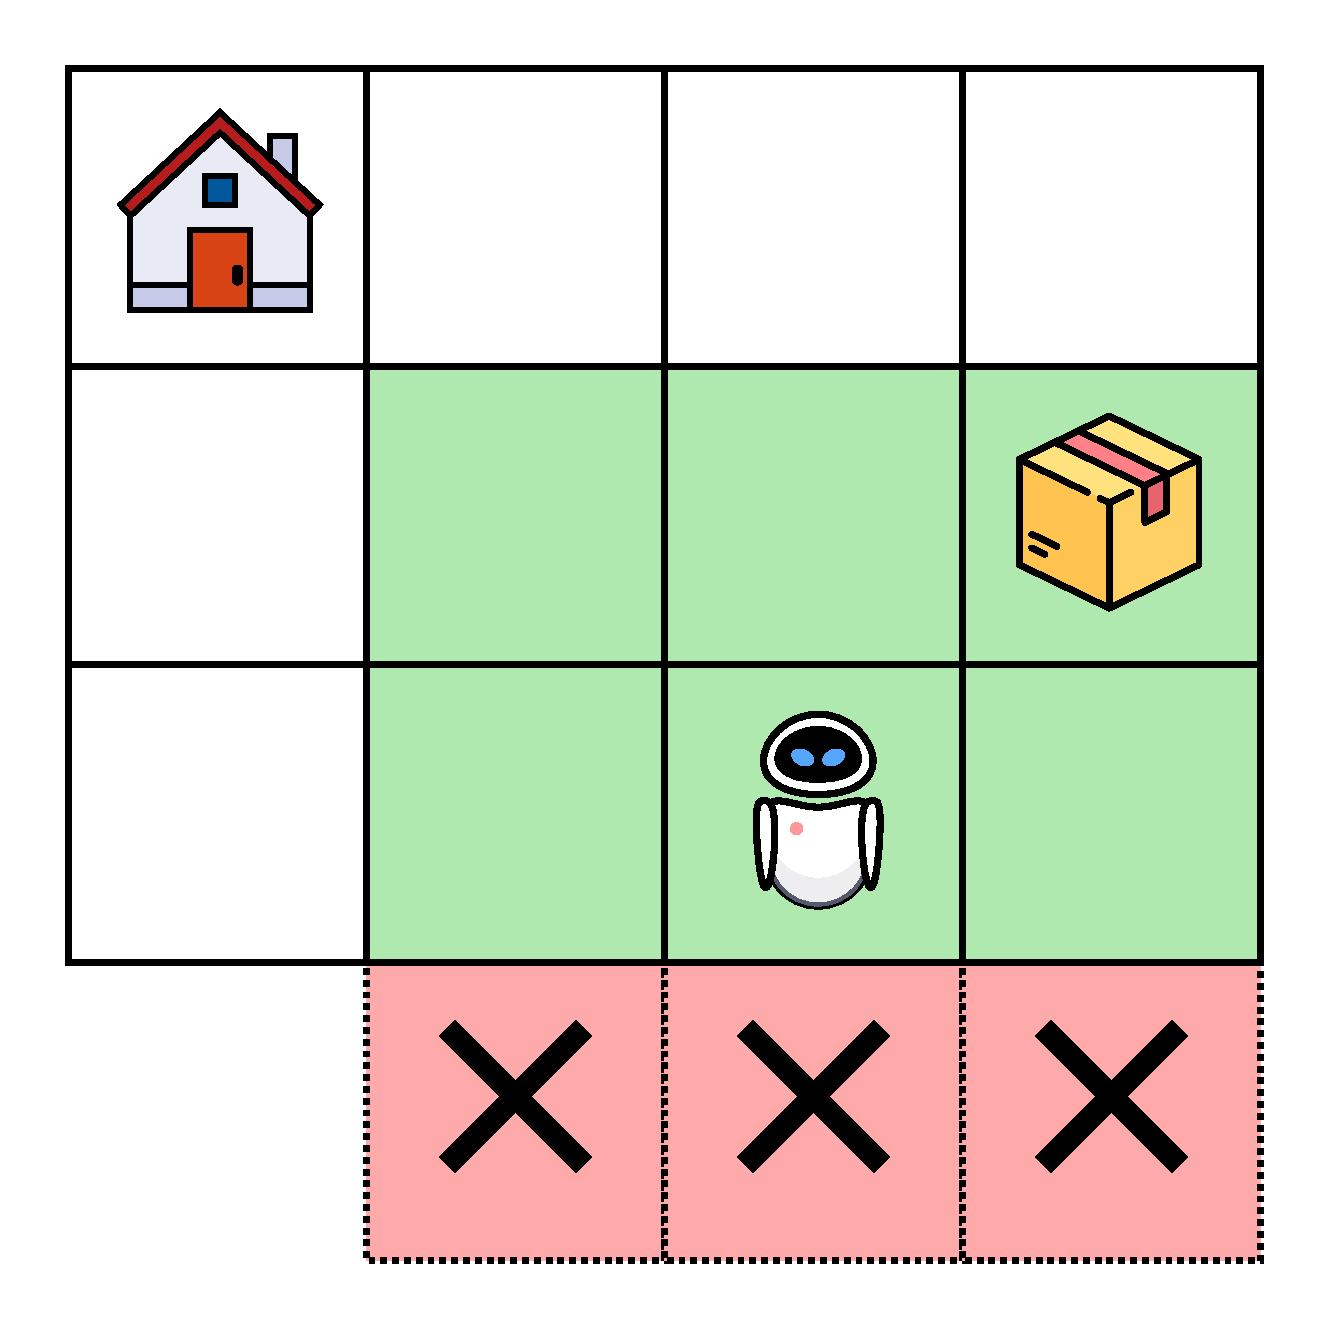
\includegraphics[height=4.5cm]{figures/world.pdf}
        \caption{Example of environment model}
        \label{fig:model}
    \end{subfigure}
    \caption{
        Environment modelling for the explorer robot domain.
        %
        The agent is in discrete bidimensional space, where it can move in eight admissible directions, namely: the cardinal ones, with north pointing up.
        %
        Direction \inlineAsl{here} denotes the current position of the agent.
    }
    \label{fig:environment-model}
\end{figure}

\subsection{Agent}\label{sec:explorer-agent}

The \texttt{ExplorerRobot} agent, whose specification is shown in~\cref{lst:agent-spec}, is designed to achieve high-level goals such as reaching a target object (e.g., “home”). It declares a set of admissible goals and beliefs that are enhanced with natural language explanations.

\lstinputlisting[
    % float,
    label={lst:agent-spec},
    caption={The \texttt{ExplorerRobot} agent as implemented in \jakta{}.},
    language=Kotlin,
    basicstyle=\scriptsize\ttfamily,
    captionpos=b,
    mathescape=false
]{listings/agent-spec.kt}

\subsection{Environment}\label{sec:explorer-environment}

The application is based on a custom grid world environment, which is implemented by extending the \texttt{Environment} class provided by \jakta{}. 
%
This environment provides two external actions for robot navigation.
%
The \texttt{Move} action enables the robot to move in a specified direction, provided that no obstacles block the path. When executed, this action reports either the success of the movement or identifies any object that the robot encounters.
%
If an obstacle prevents movement, the action has no effect.
%
The \texttt{GetDirectionToMove} action assists with navigation by binding a provided variable to a randomly selected direction free of obstacles.
%
If no directions are available for movement, the action produces no result.
%
The environment generates percepts following the format shown in~\cref{lst:gridworld-percepts}.
%
The complete environment specification is detailed in~\cref{lst:env-spec}. 
%
These percepts provide information about the robot's surroundings, including known directions and objects, obstacles that include grid borders, free cells, and the presence of objects in the eight cells that surround the agent's current position.

\begin{lstlisting}[
    basicstyle=\scriptsize\ttfamily,
    captionpos=b,
    caption={The set of percepts generated by the grid world environment.},
    label={lst:gridworld-percepts},
    breaklines=true,
]
direction(north)
object(house)
object(box)
free(north).
free(north_west).
free(north_east).
free(west).
free(east).
obstacle(south).
obstacle(south_west).
obstacle(south_east).
there_is(box, north_east).
\end{lstlisting}

\lstinputlisting[
    % float,
    label={lst:env-spec},
    caption={Specification of the grid world environment in \jakta{}.},
    language=Kotlin,
    basicstyle=\scriptsize\ttfamily,
    captionpos=b,
    mathescape=false
]{listings/env-spec.kt}

\section{Experimental Methodology}\label{sec:exp-methodology}

The evaluation employs the explorer robot application (\S~\ref{sec:exp-robot}) to assess the \ac{PGP} capabilities with different sets of parameters. 
%
The experiment consists of a square grid world with five cells along each axis containing three static obstacles, with an explorer robot agent initially positioned at the center and a target \inlineAsl{home} object located at one corner of the grid.
%
The \inlineAsl{home} object is positioned beyond the agent's initial perception range, and obstacles are placed to prevent direct navigation paths. 
%
The agent begins with the goal \inlineAsl{reach(home)} but lacks any initial plan to achieve this objective. 

Individual experiments are launched by an evaluation script (\S~\ref{sec:exp-setup}), using one of the selected language models (\S~\ref{sec:chosen-llms}) configured with predetermined parameters (\S~\ref{sec:generation-parameters}) to generate plans within a fixed timeout period.
%
The evaluation framework measures both plan validity---whether the \ac{PGP} successfully generates executable plans using available actions to reach the target---and plan quality, through metrics detailed in~\cref{sec:metrics}. 

\subsection{Experimental Setup}\label{sec:exp-setup}

Running \acp{LLM} demands substantial computational power, that puts them beyond the reach of typical consumer hardware.
%
This reality has spawned the ``\ac{LLM}-as-a-Service'' ecosystem, where providers offer model access through web APIs rather than local deployment.
%
The landscape includes established players like OpenAI's Platform API and community-driven platforms like Hugging Face, alongside aggregators such as \href{https://openrouter.ai/}{OpenRouter} that provide unified access to multiple models from different providers. 
%
To conduct the experiments, the OpenRouter's API is selected as the primary interface since its unified endpoint structure eliminates the complexity of managing multiple provider-specific integrations, easing systematic comparisons across different models. 

To assess the quality of generated plans, an automated evaluation procedure is devised based on the chosen APIs and evaluation metrics.
%
A DVC~\cite{ruslan_kuprieiev_2025_15646974} pipeline and \href{https://gradle.org/}{Gradle} tasks are used to automate the execution of a MAS for each experimental configuration to be tested and to store the results to a \href{https://dagshub.com/rbattistini/plan-generation-experiments}{remote server}.
%
In order to have a reference ground truth for the evaluation, a human baseline is provided that represents the optimal plans to achieve the goal of reaching home, which are shown in~\cref{lst:human-baseline}.

\lstinputlisting[
    % float,
    label={lst:human-baseline},
    caption={Set of baseline plans for the ExplorerRobot agent},
    language=Kotlin,
    basicstyle=\footnotesize\ttfamily,
    captionpos=b,
    mathescape=false
]{listings/baselineplans.kt}

\subsection{Language Models}\label{sec:chosen-llms}

The experiments are based on these \ac{LLM}s: \texttt{Gpt-4.1}, \texttt{Gemini 2.5 Flash}, \texttt{Deepseek Chat V3}, and \texttt{Claude Sonnet 4}.
%
They are selected based on their state-of-the-art performance, as well as for their accessibility through public APIs with no exhaustivity claim.

\subsection{Experiments' Parameters}\label{sec:generation-parameters}

The only parameters that were explicitly set are the temperature and the max tokens.

\paragraph{Temperature.}  The effect of temperature on plan generation was examined using three values: 0.1, 0.5, and 0.9. 
%
It was hypothesized that very low temperatures (0.1) would produce overly rigid outputs lacking the flexibility needed for novel objectives or ambiguous scenarios.
%
Conversely, high temperatures (0.9) were anticipated to risk compromising output quality through incoherent or hallucinatory responses, as suggested by findings in~\cite{holtzmanCuriousCaseNeural2020}.

\paragraph{Max Tokens.} The maximum token limit of 2048 is chosen to ensure that the model can generate complete and contextually rich \ac{BDI} plans.
%
Shorter limits were avoided to risk premature truncation. 
%
Longer ones were not considered useful given the limited complexity of the task.

\paragraph{Prompt Type.} Three distinct prompting strategies are evaluated to assess their impact on plan generation. 
%
The baseline approach excludes all natural language specifications, providing minimal context.
%
The intermediate strategy keeps developer-provided hints and removes the remarks.
%
The last approach preserves both hints and remarks, delivering the richest contextual information including environment-specific insights and action usage instructions. 
%
Hints and remarks were considered separately to assess how much different types of contextual information would influence the quality and effectiveness of the generated plans.

\subsection{Evaluation Metrics}\label{sec:metrics}

\begin{table}[ht]
\centering
\begin{tabularx}{\linewidth}{@{} l l X @{}}
\toprule
\textbf{Code} & \textbf{Metric} & \textbf{Description} \\
\midrule
\PC  & Plan Count               & Total number of generated plans. \\
\CC  & Context Complexity       & Average number of beliefs per plan context. \\
\PBC & Plan Body Complexity     & Average number of operations per plan body. \\
\GR  & Generalization Count     & Number of generated plans using variables rather than constants. \\
\RR  & Redundancy Amount        & Number of useless plans (e.g., not executable or subsumed). \\
\NGC & Novel Goal Count         & Number of newly-invented goals. \\
\NBC & Novel Belief Count       & Number of newly-invented beliefs. \\
\GSA & Goal Semantic Alignment  & Number of semantically-misaligned admissible goals. \\
\BSA & Belief Semantic Alignment& Number of semantically-misaligned admissible beliefs. \\
\TSR & Task Success Rate        & Percentage of experiments where the agent achieves the \inlineAsl{!reach(home)} goal. \\
\GAT & Goal Achievement Time    & Average steps required to reach the goal in successful runs. \\
\bottomrule
\end{tabularx}
\caption{Evaluation metrics for generated plans.}
\label{tab:metrics}
\end{table}

To evaluate the quality of generated plans, the metrics shown in \cref{tab:metrics} are employed.
%
Among these metrics, \GR{} and \TSR{} should be maximized (higher values are better), while \RR{}, \GSA{}, \BSA{}, \GAT{} should be minimized (lower values are better).
%
The remaining metrics (\PC{}, \CC{}, \PBC{}, \NGC{}, and \NBC{}) have no clear optimization direction, yet they provide valuable comparative insights, with both extremely low and high values potentially indicating issues.

Additionally, to establish a comprehensive evaluation metric for plan quality, the \textbf{Plan-Reference Alignment Score (\PRAS{})} metric is introduced, to compare generated plans against the human baseline.
%
For this evaluation, a \ac{LLM} is employed as an explicit judge~\cite{DBLP:journals/corr/abs-2412-05579} to assess the generated plans across three key dimensions: quality of abstraction, generalizability, and adherence to BDI principles. 
%
The \ac{LLM} judge compares these generated plans against reference implementations to provide systematic evaluation---the prompt employed for the judge is shown in~\cref{lst:llm-judge-prompt}.
%
This \ac{LLM}-as-judge methodology allows to systematically rate plan quality using criteria that would be difficult to formalize through traditional metrics alone.
%
\PRAS{} tends to one when the generated plans are similar to the reference ones, to zero when they are completely different.

\begin{lstlisting}[
    basicstyle=\scriptsize\ttfamily,
    breaklines=true,
    captionpos=b,
    caption={Prompt used for the LLM-as-judge evaluation.},
    label={lst:llm-judge-prompt},
]
"Extract invented goals, beliefs, and plans from the 'actual output'.",
"Compare extracted plans against 'expected output' plans for logical equivalence and coverage.",
"Assess if invented goals/beliefs are necessary or add needless complexity compared to 'expected output'.",
"Evaluate plan minimality; penalize unnecessary subgoals, conditions, or operations vs 'expected output'.",
"Verify that operations correctly use specified prefixes (execute, achieve, add, etc.) and admissible actions.",
"Check if conditions logically correspond to the intended plan activation scenario.",
"Score based on plan correctness, necessity of inventions, and adherence to minimality principle."
\end{lstlisting}

\section{Experimental Results}\label{sec:exp-results}

Each of the four chosen \acp{LLM} was queried ten times to account for the stochastic nature of \ac{LLM} responses, for each of the three prompting configurations and for each of the three temperature values, yielding three hundred sixty total experimental runs.

The average amount of input tokens was 995, with a min of 808 and a max of 1196.
%
The variability is due to presence of instances where multiple \acp{PGP} are invoked, so the total count is not always the number of tokens of the initial input prompt.
%
The average amount of output tokens is 223, with a min of 77 and a max of 553.
%
The average latency of the responses from OpenRouter was of 1471 ms, with a min of 288 ms and a max of 6120 ms.
%
The cost to run the experiments was approximately of one USD.
%
Note that Deepseek was offered free of charge.

Only in eight instances more than one PGP was invoked, and it never resulted in plans that reached home.
%
In this subset of experiments the PGP was called two times on average, with a single outlier in which the PGP was called nine times.
%
The rest of analysis will omit instances where the PGP was invoked more than one time.

Work in progress.

\chapter{Conclusion}\label{chap:conclusion}

This thesis focuses on the integration of \ac{GenAI} into the \agentspeak{} agent architecture to generate new plans at runtime, based on the agent's current knowledge.
%
The goal is to assess if and how \acp{LLM} can generate plans for \ac{BDI} agents, potentially reducing reliance on human programmers or first-principle planners.

Unlike approaches that treat agents as generative systems themselves, this work preserves the strengths of the \ac{BDI} model---its theoretical foundation, programming paradigms, and controllability---while enhancing it with generative and \ac{NLP} capabilities for plan generation.
%
The approach encapsulates the \ac{LLM} within a \ac{PGP} functionality, responsible for generating plans reactively or on-demand, ensuring compatibility with the \ac{BDI} architecture.
%
This thesis defines the \ac{PGP} interface, proposes implementation guidelines, and evaluates a prototype implementation to validate the approach.

Addressing~\cref{rq:required-info}, the \ac{PGP} is defined to use structured prompts detailing current and generally \emph{admissible} goals and beliefs, available actions and plans, and the operational semantics of the \ac{BDI} architecture.

For~\cref{rq:knowledge-transfer}, structured prompts paired with parsable outputs ensure reliable integration of generated plans into the agent's library, balancing expressiveness with formal rigor.
%
As experimental results confirm, providing additional semantics to the \ac{LLM} via natural language descriptions of the agent's goals, beliefs, and actions has a critical impact on the effectiveness of the LLM-based PGP, along with the application of prompt engineering best practices and appropriate sampling parameters.

Consequently, answering~\cref{rq:agent-spec}, automatic plan generation shifts the agent specification from exhaustive plan encoding to providing the basic (procedural) knowledge necessary for the problem domain, potentially leaving to the \ac{LLM} the task of handling corner cases and unexpected situations.
%
The agent operation stays the same of a classic \ac{BDI} agent, with the possibility of the \ac{PGP} to be triggered explicitly (on-demand) or implicitly (reactively) to handle goals with no matching plans.

For~\cref{rq:reusability}, the methodology outlined in this work shows promise for the generation of reusable, general plans involving variables, despite variability in \ac{LLM} performance.

In conclusion, this thesis bridges traditional \ac{BDI} architectures and emerging \ac{GenAI} technologies, laying the groundwork for more autonomous and explainable cognitive agents and opening several promising research directions.

\section{Future Work}

Future work includes exploring runtime validation and verification mechanisms to address hallucinations or inaccuracies in \ac{LLM}-generated constructs.
%
Several other research directions might be explored, including plan repair and refinement mechanisms (\S~\ref{sec:plan-repair}), experimentation with different structured output formats (\S~\ref{sec:llm-gen-formats}), enhanced modularization of BDI agent cycles (\S~\ref{sec:modularity}), integration with \ac{MCP} (\S~\ref{sec:mcp-integration}), finetuning (\S~\ref{sec:finetuning}) and use of artifacts (\S~\ref{sec:artifacts}).

Additionally, studying prompt robustness under varying conditions and developer inaccuracies could enhance the methodology's practicality.
%
Ablation studies may clarify factors influencing prompt effectiveness~\ref{rq:required-info} and knowledge transfer~\ref{rq:knowledge-transfer}.
%
Testing scenarios with concurrent goals, dynamic environments, and partial observability will validate scalability and generalization~\ref{rq:reusability}.

\subsection{Plan repair and refinement mechanisms}\label{sec:plan-repair}

Mechanisms such as plan repair, failure learning, and adaptive refinement can enhance agent autonomy and long-term performance.
%
One effective strategy involves incorporating feedback from external entities.
%
This has been successfully employed to back-prompt \acp{LLM} for improved plan generation.

As an example Voyager uses the feedback from Minecraft to provide the \ac{LLM} with up-to-date information on how the environment changed in response to its chosen actions and whether syntax errors led to failure in executing plans~\cite{WangX0MXZFA24}.
%
Analogously, Kambhampati et al.~\cite{kambhampatiLLMsCantPlan2024} demonstrate that within the LLM-Modulo framework, incorporating external verifiers or critics can significantly enhance the planning capabilities of language models.
%
Their view is encapsulated in the assertion: ''\acp{LLM} cannot plan themselves but can play a variety of constructive roles in solving planning tasks---especially as approximate knowledge sources and candidate plan generators in so-called LLM-Modulo Frameworks, where they are used in conjunction with external sound model-based verifiers``~\cite{kambhampatiLLMsCantPlan2024}.
%
This approach highlights the use of \acp{LLM} as generators of candidate solutions, with their correctness checked through independent verification mechanisms.
%
In this context, BDI engines are particularly well-suited to serve as verifiers, offering detailed feedback on the execution of \ac{LLM}-generated plans.

\subsection{Structured Output Formats}\label{sec:llm-gen-formats}

YAML was chosen as the structured format for plan generation due to the ease with which it can be parsed and its readability, which is greater than the one of XML or JSON.
%
Additionally, the format's prevalence in training data, for example through configuration files, was hypothesized to result in more reliable generation compared to specialized agent programming languages like \agentspeak{}. 

Future work with controlled natural languages~\cite{kuhnSurveyClassificationControlled2014} might be a promising direction for improving plan generation while addressing current limitations. 
%
Natural language alternatives could potentially offer higher generation quality due to training data alignment---since the vast majority of LLM training corpora consists of natural language text from books, articles, and web content rather than structured formats---potentially increasing the quality of the generated plans.
%
This alignment also facilitates easier human review and modification, and better domain expertise integration through natural descriptions, though at the cost of more complex parsing. 

Prompting with grammatical patterns could significantly improve parsing reliability, for example, by using standardized phrasings like ``when attempting to achieve [goal] given [conditions], execute [actions]'' that map deterministically to BDI constructs.
%
Template-based controlled generation represents a complementary avenue, where LLMs fill structured natural language templates that encode BDI semantics while maintaining readability, potentially combined with constraint-based generation that enforces grammatical rules as part of the generation process.
%
For what concerns this work, the choice of using YAML prioritizes the integration with the BDI interpreter over the theoretical advantages of native agent programming language output or the contextual richness of natural language planning descriptions.

\subsection{Improved Software Modularity}\label{sec:modularity}

\paragraph{Plan Generation.} Despite all the LM-related logic being implemented in a separate module, the PGP is still tightly coupled with the BDI engine.
%
The sense-reason-act cycle of a BDI agent  could be further decomposed into pluggable components to support dynamic composition and substitution of agent functionalities through external modules. 
%
This approach would enable users to define in a declarative way how an agent's cognitive cycle is composed as part of its specification, e.g.\ what component to use for plan selection or for running intentions.
%
This modular architecture would make it easier to separate all plan generation functions from the BDI engine.
%
This means plan generation could be integrated by adjusting the deliberation phase to handle cases where no plan is available and enhancing the action phase to manage \texttt{GeneratePlan} and \texttt{TrackGoalExecution} goals.

\paragraph{Logging System.} The current logging implementation is tightly coupled with the BDI engine. An event-driven architecture can be implemented, by leveraging Kotlin Flows, to define a separate logging module that registers as a listener for events emitted by the BDI engine.

\subsection{Model Context Protocol Integration}\label{sec:mcp-integration}

A promising direction for enhancing \ac{LLM}-augmented \ac{BDI} agent systems involves leveraging \ac{MCP}, an open standard that enables to build connections between data sources and GenAI-powered applications.

Unlike the current implementation of the \ac{PGP}, which requires custom interfaces for each external tool or data source the BDI agent accesses---such as the logic to retrieve the agent's context---\ac{MCP} provides a standardized, reusable mechanism to integrate diverse components.

\ac{MCP} facilitates the construction of flexible, composable pipelines that orchestrate retrieval, transformation, and reasoning components. 
%
This enables more sophisticated plan-generation workflows, where the \ac{LLM} can draw from heterogeneous sources such as knowledge graphs, databases, reasoning tools, or other APIs.

An potential application of this approach is to integrate with a \ac{MCP} server that performs \ac{RAG}. 
%
This can help reduce the size of the \ac{LLM} prompt, which in turn improves inference times and reduces token consumption. 
%
Instead of passing the entire agent context to the \ac{LLM}, the \ac{RAG} pipeline would extract only the most relevant subset, based for example on the current goal or plan-in-progress.

Furthermore, the same \ac{MCP}-based infrastructure could enable the \ac{LLM} to reason over execution traces of other agents---e.g., to detect cooperative or competitive behaviors and act accordingly. 
%
Specialized \ac{MCP} connectors could expose the agent's belief base, intention stack, and historical plans as structured knowledge.

This architecture would not only improve the performance and adaptability of \ac{LLM}-enhanced BDI agents but also enable better reuse, composability, and scalability across a range of agent configurations and environments.

\subsection{Finetuning Small Language Models}\label{sec:finetuning}

An advantage of the proposed PGP is that it works with pretrained LLMs without any kind of finetuning.
%
That said, it is worth considering the opportunity of finetuning \acp{SLM}, especially since with current state-of-the-art models results seem promising.

Domain-specific finetuning could significantly improve plan generation quality for specialized applications. 
%
Training on curated datasets of high-quality plans in specific domains can enhance the model's understanding of domain constraints, best practices, and common failure modes.

Using \acp{SLM} instead of large-scale \acp{LLM} also offers notable advantages in terms of efficiency and speed since \acp{SLM} are faster and less resource-intensive.

\subsection{Artifacts as Tools}\label{sec:artifacts}

Future developments could explore the incorporation of artifacts---and more specifically, cognitional artifacts---as a means to further structure the interaction between generative \ac{BDI} agents and the environment.

Artifacts in the \aaa{} are computational entities designed to be used by agents, exposing functionality through a well-defined \textit{usage interface}, and optionally enriched with \textit{function descriptions} and \textit{operating instructions}.
%
These features make artifacts naturally compatible with \acp{LLM}, as they embody a set of properties increasingly characteristic of \ac{LLM}-native software development.

Artifacts provide \textit{introspectability} by exposing their purpose and usage in a form that can be reasoned about symbolically or through language.
%
They offer \textit{explainability} through function and operation descriptions that can be explicitly described in natural language, making them amenable to \ac{LLM} understanding and debugging. 
%
Additionally, artifacts provide \textit{modularity} by offering encapsulated, reusable functionality that could be invoked or composed by \ac{LLM}-generated plans.

Recent trends in GenAI highlight the shift toward language-accessible software, where components are made self-descriptive and navigable by \acp{LLM}. 
%
Cognitional artifacts---by design---already promote this pattern, and could serve as interfaces or tools that \acp{LLM} can select, understand, and use during plan generation.

As such, a promising future direction is the development of artifact-based infrastructures in which \acp{LLM} reason over available artifacts via their function descriptions, generate plans informed by artifact operating instructions, and execute them through artifact usage interfaces.

This would also support a more declarative, open-ended, and cognitively rich model of agent behavior, aligning with the \textit{Agens Faber} vision, where agent intelligence includes the capacity to understand, use, and even construct new artifacts.

\chapter*{Acknowledgements}

I would like to thank my supervisor Giovanni Ciatto and cosupervisor Gianluca Aguzzi, for their guidance and support throughout this thesis.
%
I am also thankful to the doctoral candidates Martina Baiardi and Samuele Burattini for their suggestions and feedback, which helped shape the research direction.
%
Additional thanks go to Professor Alessandro Ricci for his insightful input during our group meetings.

Last but not least, I want to thank my family for their support, patience, and encouragement throughout this master's program.

%----------------------------------------------------------------------------------------
% BIBLIOGRAPHY
%----------------------------------------------------------------------------------------

\backmatter%
\printbibliography[heading=bibintoc]%

\end{document}